\documentclass{beamer}
%\usetheme{Boadilla}
%\usetheme{Szeged}
%\usetheme{Singapore}
\usetheme{Frankfurt}
\usecolortheme{dove}
\newenvironment{alltt}{\ttfamily}{\par}
\usepackage{amsmath,amssymb,amsfonts,amsthm, multicol, subfigure, color}
\usepackage{bm}
\usepackage{graphicx}
\usepackage{tabularx}
\usepackage{booktabs}
\usepackage{hyperref}
\usepackage{pdfpages}
\definecolor{dodgerblue}{rgb}{.118, .575, 1}
\def\independenT#1#2{\mathrel{\rlap{$#1#2$}\mkern2mu{#1#2}}}
\newcommand\independent{\protect\mathpalette{\protect\independenT}{\perp}}
\newcommand\indep{\protect\mathpalette{\protect\independenT}{\perp}}
\def\logit{\text{logit}}
\usepackage{stackrel}
\usepackage{tikz}
\usetikzlibrary{arrows,shapes.arrows,positioning,shapes}
\newcommand\red[1]{{\color{red}#1}}
\newcommand\bred[1]{{\color{red}\textbf{#1}}}
\newcommand\blue[1]{{\color{blue}#1}}
\newcommand\bblue[1]{{\color{blue}\textbf{#1}}}
\newcommand\green[1]{{\color{olive}#1}}
\newcommand\bgreen[1]{{\color{olive}\textbf{#1}}}
\newcommand\purple[1]{{\color{purple}#1}}
\newcommand\orange[1]{{\color{orange}#1}}
\newcommand\black[1]{{\color{black}#1}}
\newcommand\white[1]{{\color{white}#1}}
\newcommand\teal[1]{{\color{teal}#1}}
\newcommand\magenta[1]{{\color{magenta}#1}}
\newcommand\Fuchsia[1]{{\color{Fuchsia}#1}}
\newcommand\BlueGreen[1]{{\color{BlueGreen}#1}}
\newcommand\iid{\stackrel{\text{iid}}{\sim}}
\newcommand\E{\text{E}}
\newcommand\V{\text{V}}
\renewcommand\P{\text{P}}
\newcommand{\tcframe}{\frame{
\small{
\only<1|handout:0>{\tableofcontents}
\only<2|handout:1>{\tableofcontents[currentsection]}}
}}
% Credit for the following to https://tex.stackexchange.com/questions/44983/beamer-removing-headline-and-its-space-on-a-single-frame-for-plan-but-keepin
\makeatletter
    \newenvironment{withoutheadline}{
        \setbeamertemplate{headline}[default]
        \def\beamer@entrycode{\vspace*{-\headheight}}
    }{}
\makeatother
\setbeamercovered{invisible}

\title{\blue{Precept 8: Missing Data}}
\subtitle{\green{Soc 504: Advanced Social Statistics}}
\author{Ian Lundberg}
\institute[Princeton]{Princeton University}
\date{April 6, 2018}

\begin{document}

\frame{\titlepage}

\begin{frame}
\frametitle{Outline}
\tableofcontents
\end{frame}

\begin{frame}{Learning goals}
By the end of precept, you should be able to:
\begin{enumerate}
\item Feel comfortable with three common \bgreen{assumptions} about missing data
\begin{itemize}
\item Missing completely at random
\item Missing at random
\item Non-ignorable
\end{itemize}
\item Be able to reason about the plausibility of these assumptions using \bgreen{substantive knowledge} in real research settings.
\item Connect assumptions to concrete \bgreen{strategies} to deal with missing data
\begin{itemize}
\item Listwise deletion
\item Multiple imputation
\item Bounds
\end{itemize}
\end{enumerate}
\end{frame}

\section{Motivation}

\begin{frame}
\frametitle{Outline}
\tableofcontents[currentsection]
\end{frame}

\begin{frame}
\begin{multicols}{2}
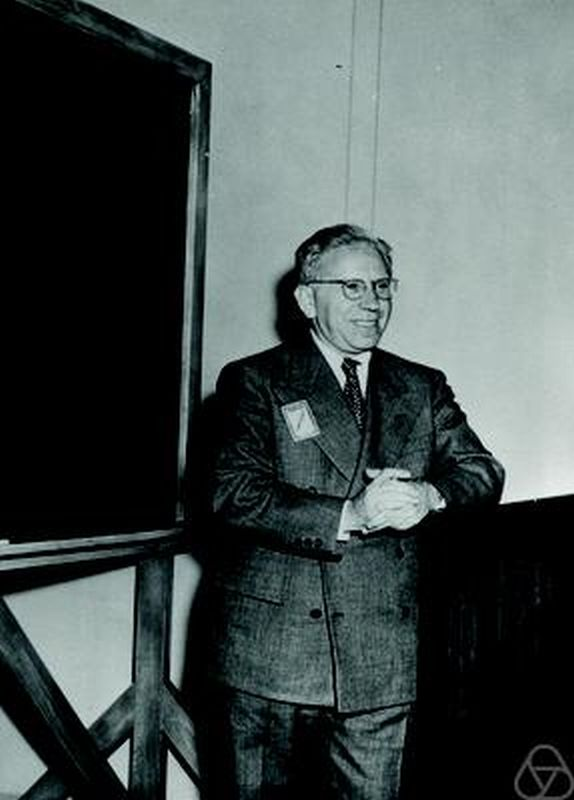
\includegraphics[width = .5\textwidth]{figs/Abraham_Wald}\footnote{PC: Wikimedia commons}

Abraham Wald 
\begin{itemize}
\item b. 1902, Austria-Hungary
\item Jewish, persecuted in WWII
\item Fled to U.S. in 1938
\item Namesake of the Wald test
\item Statistical consultant for U.S. Navy in WWII
\end{itemize}
\end{multicols}
\end{frame}

\begin{frame}
\textcolor{blue}{Question:} Where should armor be added to protect planes? \vskip 1cm
\textcolor{blue}{Data:} Suppose we saw the following planes.\footnote{Story told by Mangel and Samaniego 1984 [\href{http://dx.doi.org/10.1080/01621459.1984.10478038}{\textcolor{blue}{link}}].\\ Presentation style inspired by Joe Blitzstein. See the original here [\href{https://www.youtube.com/watch?v=dzFf3r1yph8}{\textcolor{blue}{link}}] \vskip .2cm}
\end{frame}

\begin{frame}{\blue{Observed data}: Planes that came home with damage}
\begin{center}
\begin{tikzpicture}[x = .5\textwidth, y = .5\textheight]
\node at (0,0) {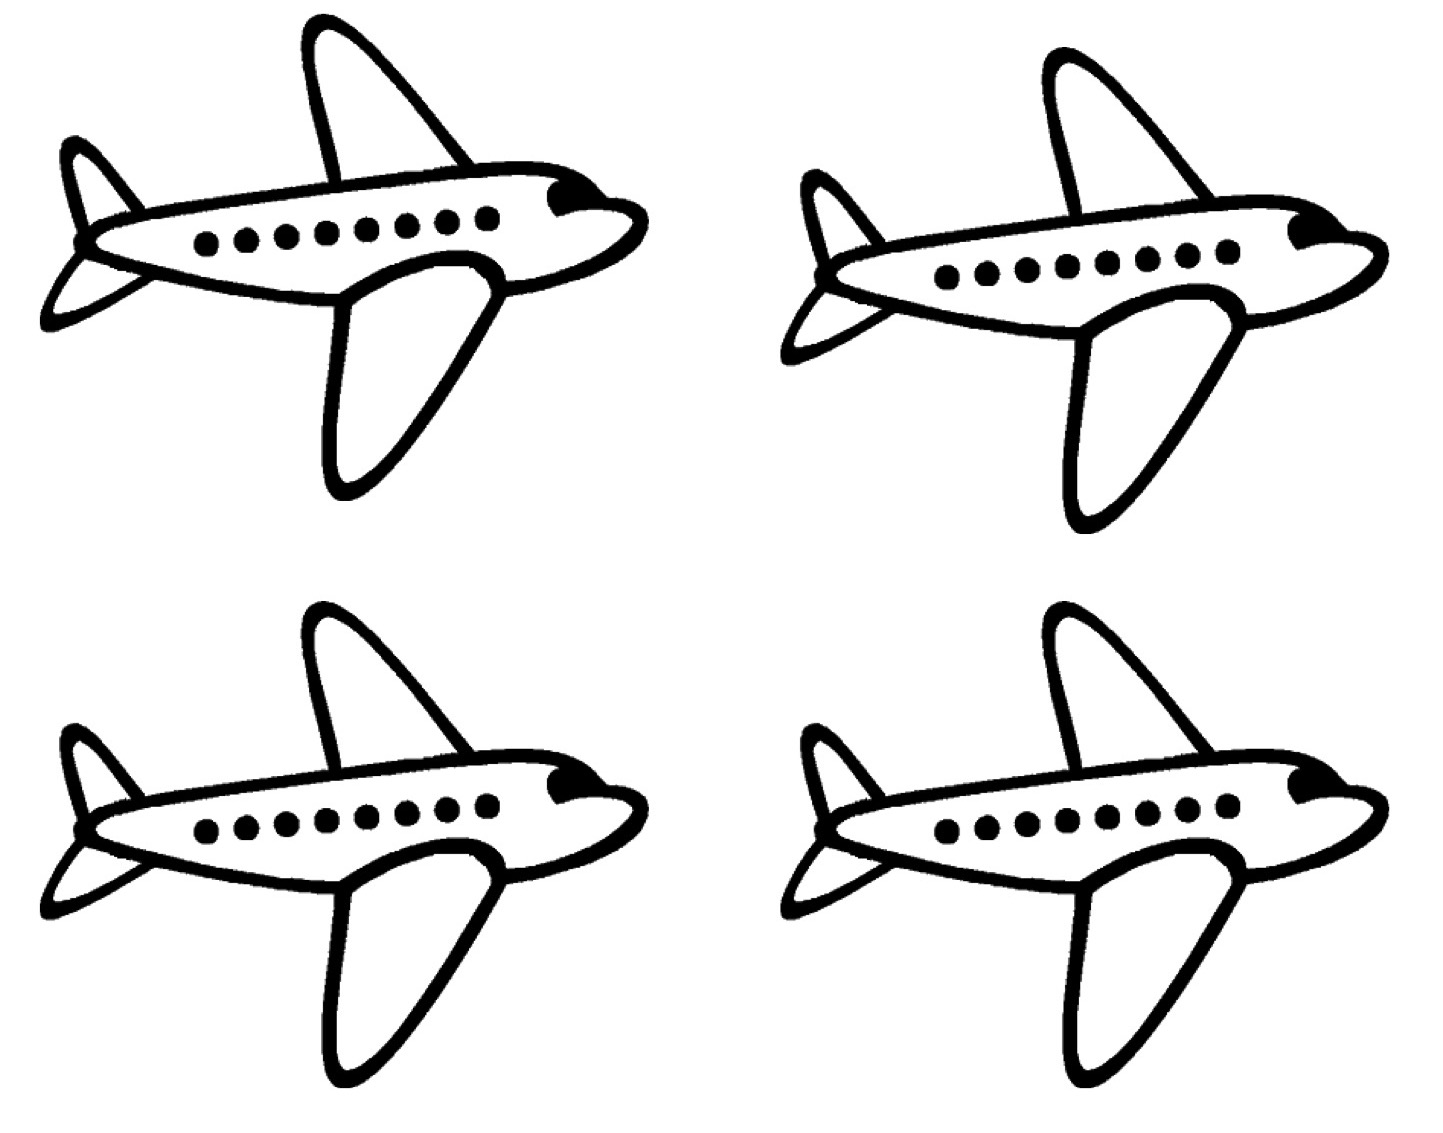
\includegraphics[width = .6\textwidth]{figs/planes.jpg}};
% Upper left plane (tail hits)
\onslide<2->{\node at (-.4,.35) {\huge \red{$\bullet$}};}
\onslide<3->{\node at (-.45,.3) {\huge \red{$\bullet$}};}
\onslide<4->{\node at (-.5,.33) {\huge \red{$\bullet$}};}
\onslide<5->{\node at (-.55,.28) {\huge \red{$\bullet$}};}
\onslide<6->{\node at (-.53,.4) {\huge \red{$\bullet$}};}
\onslide<7->{\node at (-.3,.3) {\huge \red{$\bullet$}};}
% Upper right plane (one wing hits)
\onslide<9->{\node at (.1,.35) {\huge \red{$\bullet$}};}
\onslide<10->{\node at (.3,.35) {\huge \red{$\bullet$}};}
\onslide<11->{\node at (.25,.28) {\huge \red{$\bullet$}};}
\onslide<12->{\node at (.4,.25) {\huge \red{$\bullet$}};}
\onslide<13->{\node at (.32,.21) {\huge \red{$\bullet$}};}
\onslide<14->{\node at (.32,.1) {\huge \red{$\bullet$}};}
% Lower left plane (body and one wing hits)
\onslide<15->{\node at (-.3,-.3) {\huge \red{$\bullet$}};}
\onslide<16->{\node at (-.5,-.3) {\huge \red{$\bullet$}};}
\onslide<17->{\node at (-.35,-.25) {\huge \red{$\bullet$}};}
\onslide<18->{\node at (-.4,-.27) {\huge \red{$\bullet$}};}
\onslide<19->{\node at (-.28,-.2) {\huge \red{$\bullet$}};}
\onslide<20->{\node at (-.3,-.1) {\huge \red{$\bullet$}};}
% Lower right plane (body hits)
\onslide<21->{\node at (.1,-.3) {\huge \red{$\bullet$}};}
\onslide<22->{\node at (.25,-.23) {\huge \red{$\bullet$}};}
\onslide<23->{\node at (.2,-.3) {\huge \red{$\bullet$}};}
\onslide<24->{\node at (.32,-.28) {\huge \red{$\bullet$}};}
\node at (0,-.8) {\Large \blue{Q:} Where would you add armor?};
\end{tikzpicture}
\end{center}
%Where should we add armor?
\end{frame}

\begin{frame}
\Huge Discussion \vskip .1cm
\bblue{Don't peek} at the next slide if you downloaded these!
\end{frame}

\begin{frame}{\blue{Missing data}: Planes that never returned}
\pause
\begin{center}
\begin{tikzpicture}[x = .5\textwidth, y = .5\textheight]
\node at (0,0) {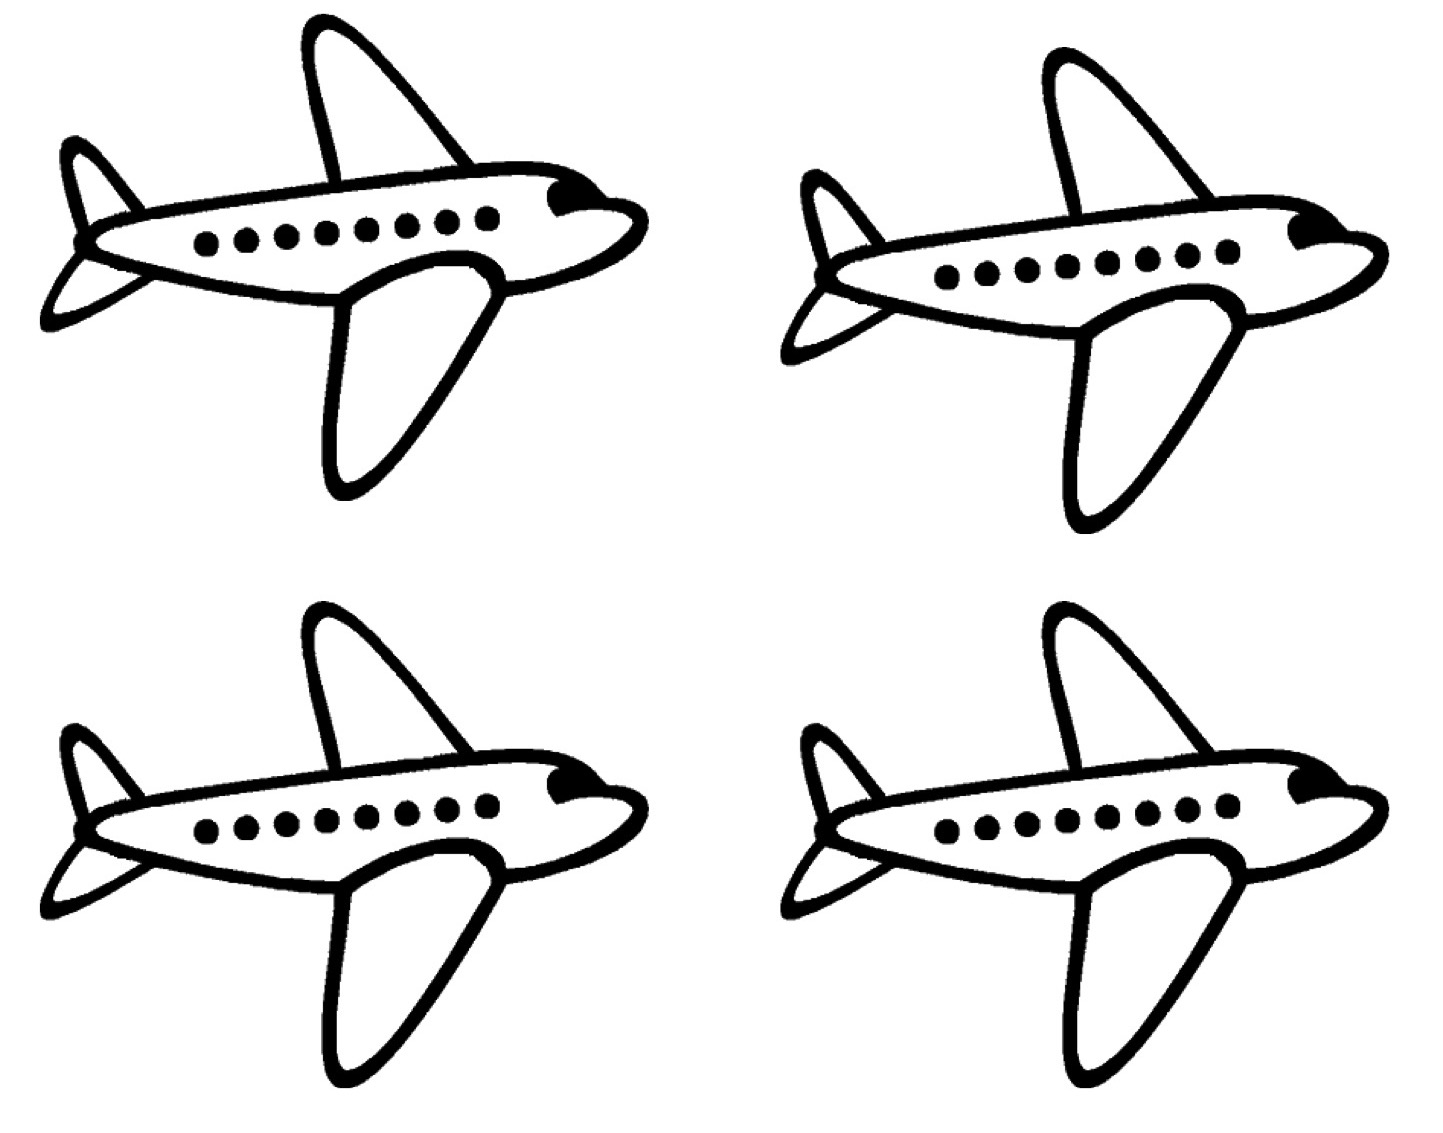
\includegraphics[width = .6\textwidth]{figs/planes.jpg}};
% Upper left plane
\node at (-.09,.34) {\huge \red{$\bullet$}};
\node at (-.14,.3) {\huge \red{$\bullet$}};
% Upper right plane
\node at (.53,.31) {\huge \red{$\bullet$}};
\node at (.47,.33) {\huge \red{$\bullet$}};
% Lower left plane
\node at (-.09,-.25) {\huge \red{$\bullet$}};
\node at (-.14,-.25) {\huge \red{$\bullet$}};
% Lower right plane
\node at (.53,-.25) {\huge \red{$\bullet$}};
\node at (.48,-.27) {\huge \red{$\bullet$}};
\end{tikzpicture}
\end{center}
\end{frame}

\begin{frame}
\large Now where should we add armor? \pause \textcolor{blue}{To the nose!} \pause \vskip 1cm
Results from the observed planes were misleading because data were \textcolor{blue}{not missing at random}! \pause \vskip .5cm
Missing data requires careful thought. \pause \vskip .5cm
\begin{center}\LARGE \blue{No algorithm solves it for you!}\end{center}
\end{frame}

\begin{frame}
We will walk through the assumptions and implementation of multiple imputation. \pause \vskip .5cm
Our example will be the \textcolor{blue}{2016 General Social Survey (GSS)}. \pause \vskip .5cm
The GSS measures Americans' attitudes toward lots of issues. \pause \vskip .5cm
List of files (we use 2016): {\footnotesize \textcolor{blue}{\url{http://gss.norc.org/get-the-data/spss}}} \\
\href{http://gss.norc.org/Documents/spss/2016_spss.zip}{\textcolor{blue}{Link}} directly to data download \vskip .5cm \pause
The GSS is a complex sample design. We will draw inferences about the \blue{sample}. In two weeks we will learn how to generalize these to the \blue{population} using weights.
\end{frame}

\begin{frame}
\bblue{Research question}:\\
\begin{center}
What is the relationship between the \\
\green{\Large respondent's education} \\
and the respondent's \\
\green{\Large father's education}? \vskip 1cm \pause
(Beyond attitudinal questions, the GSS asks several questions related to \blue{mobility})
\end{center}
\end{frame}

\begin{frame}
\texttt{paeduc} captures father's education in years. \pause \vskip .2cm
But it's sometimes missing. \textcolor{blue}{We need to know why!}\vskip .2cm
\begin{center}
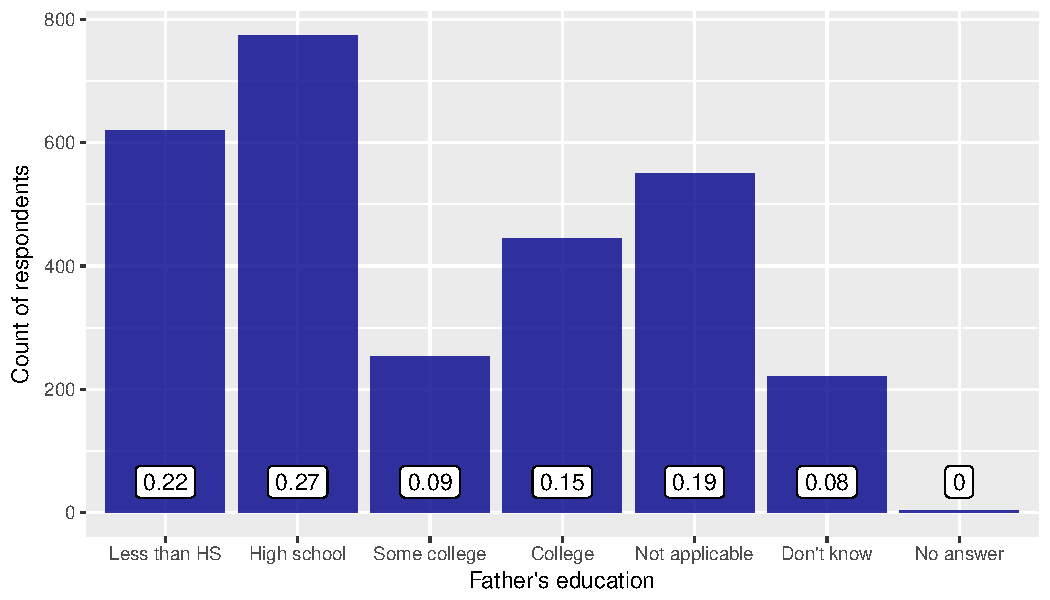
\includegraphics[width = .8\textwidth]{figs/PaEduc.pdf}
\end{center}
\end{frame}

\begin{frame}
Why is father's education missing? \vskip .5cm
Check the codebook (p. 176) [\href{https://gssdataexplorer.norc.org/documents/440/display}{\textcolor{blue}{link}}] \vskip .5cm
\begin{center}
\includegraphics[width = .8\textwidth]{figs/paeduc_codebook}\end{center} \vskip .5cm
These are the \bgreen{``Not applicable''} cases. \vskip .2cm
You should \textcolor{blue}{always} know what your variables are!
\end{frame}

\begin{frame}{Questionnaire logic, graphically}
\begin{scriptsize}
\begin{center}
  \begin{tikzpicture}[x = 2cm, y = 1cm]
  \node (placeholder) at (5,-4) {};
  \node[align=center] (F) at (0,0) {Was father in\\household\\at age 16?};
  \node (Y1) at (1,0) {Yes};
  \node (N1) at (0,-1) {No};
  \node[align=center] (Result1) at (4,0) {\only<2->{Father's\\education}};
  \node[align=center] (OM) at (1,-1) {\only<3->{Was another male\\in household?}};
  \node (Y2) at (2,-1) {\only<3->{Yes}};
  \node (N2) at (1,-2) {\only<3->{No}};
  \node[align=center] (Result2) at (4,-1) {\only<4->{Other male's\\education}};
  \node[align=center] (Result3a) at (4,-2) {\only<5->{\bgreen{Not applicable}}};  \draw[->, >=stealth, thick] (F) -- (Y1);
  \draw[->, >=stealth, thick] (F) -- (N1);
  \path <2-> [->] (Y1) edge (Result1);
  \path <3-> [->] (N1) edge (OM);
  \path <3-> [->] (OM) edge (Y2);
  \path <3-> [->] (OM) edge (N2);
  \path <4-> [->] (Y2) edge (Result2);
  \path <5-> [->] (N2) edge (Result3a);
  \end{tikzpicture}
\end{center}
\end{scriptsize}
We must decide what to do with the not applicable, don't know, and no answer cases.
\end{frame}

\section{Listwise deletion}
\tcframe

\begin{frame}{Listwise deletion}

We could just \blue{drop anybody with missing values}. \pause

% latex table generated in R 3.4.3 by xtable 1.8-2 package
% Mon Apr  2 21:25:42 2018
\begin{table}[ht]
\centering
\begingroup\scriptsize
\begin{tabular}{lccccc}
 & \multicolumn{5}{c}{Father's education (total $N = 2,630$)} \\
 \cmidrule(lr){2-6}
 Respondent's \\
 education & Less than HS & High school & Some college & College & \bred{MISSING} \\ 
 \cmidrule(lr){1-1} \cmidrule(lr){2-6}
College & 122 & 230 & 119 & 280 & \red{135} \\ 
  Some college & 146 & 184 &  65 &  76 & \red{164} \\ 
  High school & 197 & 246 &  33 &  41 & \red{227} \\ 
  Less than HS & 122 &  48 &  11 &   7 & \red{168} \\ 
   \hline
\bred{MISSING} &   \red{1} &   \red{2} &   \red{0} &   \red{0} &   \red{6} \\
  \end{tabular}
  \endgroup
  \caption{GSS data on respondent's and father's education: Sample counts}
\end{table}
\end{frame}

\begin{frame}
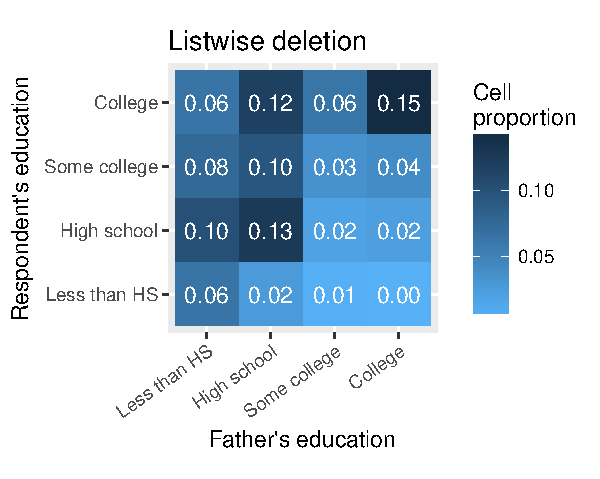
\includegraphics[width = .8\textwidth]{figs/mobility_table_listwise_deletion} \vskip .5cm \pause
\bblue{Q:} Under \bblue{what assumption} are these estimates unbiased?
\end{frame}

\begin{frame}{Missing Completely at Random (MCAR)}
\centering
  Data are missing completely at random if \blue{$\P(M\mid X) = \P(M)$} \vskip .2cm
  \begin{table}[ht] \pause
\centering
\begingroup\tiny
\begin{tabular}{lccccc}
 & \multicolumn{5}{c}{Father's education (total $N = 2,630$)} \\
 \cmidrule(lr){2-6}
 Respondent's \\
 education & Less than HS & High school & Some college & College & \bred{MISSING} \\ 
 \cmidrule(lr){1-1} \cmidrule(lr){2-6}
College & 122 & 230 & 119 & 280 & \red{135} \\ 
  Some college & 146 & 184 &  65 &  76 & \red{164} \\ 
  High school & 197 & 246 &  33 &  41 & \red{227} \\ 
  Less than HS & 122 &  48 &  11 &   7 & \red{168} \\ 
   \hline
\bred{MISSING} &   \red{1} &   \red{2} &   \red{0} &   \red{0} &   \red{6} \\
  \end{tabular}
  \endgroup \pause
  %\caption{GSS data on respondent's and father's education: Sample counts}
\end{table} \vskip .2cm
  In this case, MCAR requires that \\
  \green{missingness is independent of the true values}\\
  of father's and respondent's education. \vskip 1cm \pause
  {\Large If data are MCAR, then listwise deletion is unbiased.}
\end{frame}

\section{Bounds}
\tcframe

\begin{frame}{Bounds}
MCAR is a strong assumption that requires \blue{substantive theory}. \vskip .2cm \pause
Could we bound some proportions with \blue{weaker assumptions}? \vskip .2cm \pause
Place an upper bound on the proportion of the sample with \blue{extreme upward mobility}:
\begin{center}
father did not complete high school \\
but respondent attained a college degree
\end{center} \pause
\resizebox{\textwidth}{!}{
  \begin{tabular}{lccccc}
 & \multicolumn{5}{c}{Father's education (total $N = 2,630$)} \\
 \cmidrule(lr){2-6}
 Respondent's \\
 education & Less than HS & High school & Some college & College & \bred{MISSING} \\ 
 \cmidrule(lr){1-1} \cmidrule(lr){2-6}
College & \bblue{122} & 230 & 119 & 280 & \red{135} \\ 
  Some college & 146 & 184 &  65 &  76 & \red{164} \\ 
  High school & 197 & 246 &  33 &  41 & \red{227} \\ 
  Less than HS & 122 &  48 &  11 &   7 & \red{168} \\ 
   \hline
\bred{MISSING} &   \red{1} &   \red{2} &   \red{0} &   \red{0} &   \red{6} \\
  \end{tabular}
}
\end{frame}

\begin{frame}
\centering
\begin{tikzpicture}[x = .5\textwidth, y = .5\textheight]
\node at (0,0) {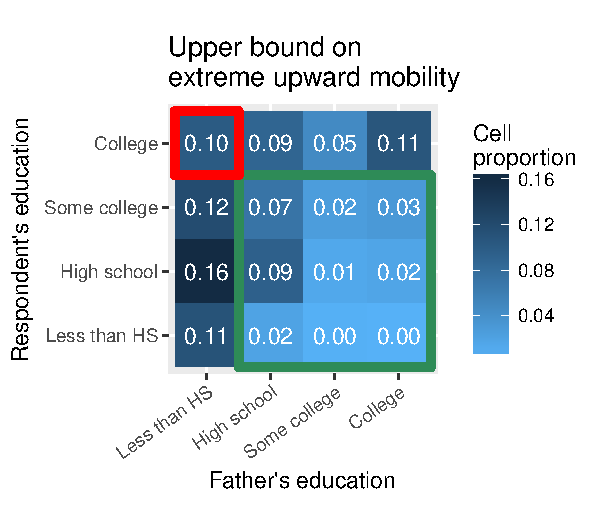
\includegraphics[width = .8\textwidth]{figs/mobility_table_upper_bound}};
\node[red] (upper) at (-.6,.65) {\textbf{Upper bound}};
\draw[->, red, line width = 2pt] (upper) to[bend right] (-.38,.47);
\node[olive] (lower) at (.55,-.5) {\textbf{Lower bound}};
\draw[->, olive, line width = 2pt] (lower) to[bend right] (.4,-.3);
\end{tikzpicture}
\end{frame}

\begin{frame}
Place an upper bound on the proportion of the sample with \blue{extreme downward mobility}: \\
\begin{center}
father completed college \\
but respondent did not complete high school
\end{center}
\resizebox{\textwidth}{!}{
  \begin{tabular}{lccccc}
 & \multicolumn{5}{c}{Father's education (total $N = 2,630$)} \\
 \cmidrule(lr){2-6}
 Respondent's \\
 education & Less than HS & High school & Some college & College & \bred{MISSING} \\ 
 \cmidrule(lr){1-1} \cmidrule(lr){2-6}
College & 122 & 230 & 119 & 280 & \red{135} \\ 
  Some college & 146 & 184 &  65 &  76 & \red{164} \\ 
  High school & 197 & 246 &  33 &  41 & \red{227} \\ 
  Less than HS & 122 &  48 &  11 &   \bblue{7} & \red{168} \\ 
   \hline
\bred{MISSING} &   \red{1} &   \red{2} &   \red{0} &   \red{0} &   \red{6} \\
  \end{tabular}
}
\end{frame}

\begin{frame}
\centering
\begin{tikzpicture}[x = .5\textwidth, y = .5\textheight]
\node at (0,0) {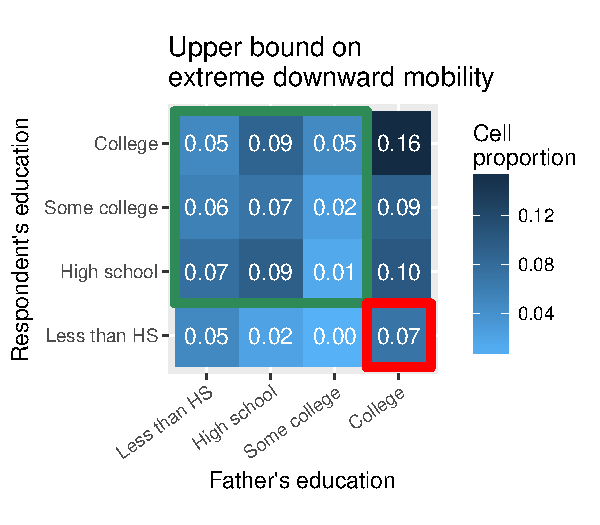
\includegraphics[width = .8\textwidth]{figs/mobility_table_lower_bound}};
\node[olive] (upper) at (-.6,.65) {\textbf{Lower bound}};
\draw[->, olive, line width = 2pt] (upper) to[bend right] (-.38,.47);
\node[red] (lower) at (.55,-.5) {\textbf{Upper bound}};
\draw[->, red, line width = 2pt] (lower) to[bend right] (.4,-.3);
\end{tikzpicture}
\end{frame}

\begin{frame}{Summarizing our bounds analysis}
\centering
\scalebox{.5}{\begin{tikzpicture}[x = .5\textwidth, y = .5\textheight]
\node at (0,0) {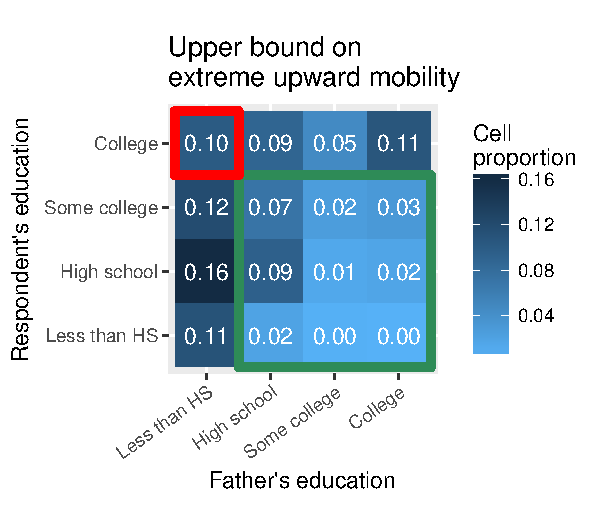
\includegraphics[width = .8\textwidth]{figs/mobility_table_upper_bound}};
\node[red] (upper) at (-.6,.65) {\textbf{Upper bound}};
\draw[->, red, line width = 2pt] (upper) to[bend right] (-.38,.47);
\node[olive] (lower) at (.55,-.5) {\textbf{Lower bound}};
\draw[->, olive, line width = 2pt] (lower) to[bend right] (.4,-.3);
\end{tikzpicture}}
\scalebox{.5}{\begin{tikzpicture}[x = .5\textwidth, y = .5\textheight]
\node at (0,0) {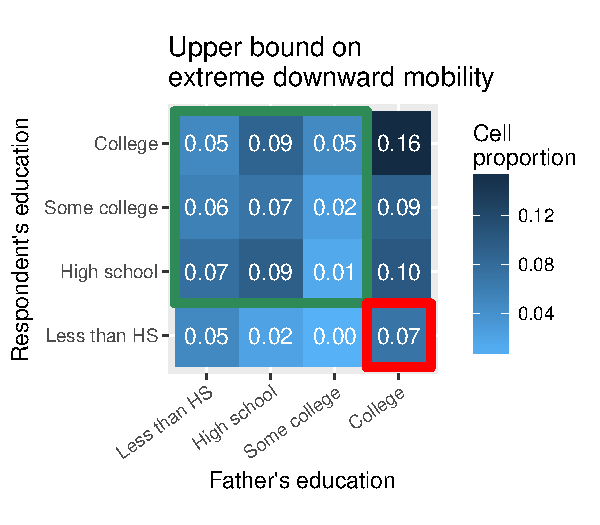
\includegraphics[width = .8\textwidth]{figs/mobility_table_lower_bound}};
\node[olive] (upper) at (-.6,.65) {\textbf{Lower bound}};
\draw[->, olive, line width = 2pt] (upper) to[bend right] (-.38,.47);
\node[red] (lower) at (.55,-.5) {\textbf{Upper bound}};
\draw[->, red, line width = 2pt] (lower) to[bend right] (.4,-.3);
\end{tikzpicture}}
\resizebox{\textwidth}{!}{
  \begin{tabular}{lccccc}
 & \multicolumn{5}{c}{Father's education (total $N = 2,630$)} \\
 \cmidrule(lr){2-6}
 Respondent's \\
 education & Less than HS & High school & Some college & College & \bred{MISSING} \\ 
 \cmidrule(lr){1-1} \cmidrule(lr){2-6}
College & 122 & 230 & 119 & 280 & \red{135} \\ 
  Some college & 146 & 184 &  65 &  76 & \red{164} \\ 
  High school & 197 & 246 &  33 &  41 & \red{227} \\ 
  Less than HS & 122 &  48 &  11 &   7 & \red{168} \\ 
   \hline
\bred{MISSING} &   \red{1} &   \red{2} &   \red{0} &   \red{0} &   \red{6} \\
  \end{tabular}
}
\end{frame}

\begin{frame}
\frametitle<+->{\bblue{Generalizing}: When can you use sharp bounds?\\(Slide adapted from materials by Brandon Stewart)}
The following gives us \blue{sharp Manski bounds} (see e.g. Aronow and Miller Chapter 4)
\begin{itemize}[<+->]
\item Assumptions:
\begin{itemize}
\item $Y_i$ is \blue{bounded} with support $[a,b]$
\item We assume stable outcomes  $Y_i^* = Y_iM_i + (\alert{\text{NA}})(1-M_i)$
\end{itemize}
\item We obtain sharp bounds for $E[Y]$ by first plugging in $a$ for all missing values to get the \blue{lower} bound, followed by plugging in $b$ for all missing values to get the \blue{upper} bound.
\item This leaves our quantity \blue{set identified} as opposed to our usual \blue{point identified}
\item Without further \blue{assumptions} we can do no better.
\item This only works with bounded support and becomes much harder with missingness on many variables
\end{itemize}
\end{frame}

\section{Multiple imputation}
\tcframe

\begin{frame}{Multiple imputation}
\blue{Multiple imputation} is a strategy to report a good \blue{point estimate} with accurate \blue{uncertainty}. \vskip .2cm \pause
If data are \bgreen{missing at random} (MAR), then multiply imputed estimates are \bgreen{unbiased}. \vskip .2cm \pause
In many (but not all) settings, MAR is more plausible than MCAR. \pause
\begin{table}
\small
\begin{tabular}{p{.5\textwidth}p{.45\textwidth}}
Missing at Random & Missing \emph{Completely} at Random \\
\hline
$\P(M\mid X_\text{Obs},X_\text{Miss}) = \P(M\mid X_\text{Obs})$ & $\P(M\mid X) = \P(M)$ \\
\\
Missingness is independent of the true values \blue{given the observed values}. & Missingness is independent of the true values. \\
\\
Implies that multiple imputation is unbiased. & Implies that listwise deletion is unbiased.
\end{tabular}
\end{table}
\end{frame}

\frame{
\frametitle{The Multiple Imputation Scheme (from lecture)}
\hspace{2em}
\pause
\begin{tikzpicture}
[overlay,inner sep = 3mm,
missdata/.style={rectangle, draw=red!50, fill=red!20, thick},
 impdata/.style={rectangle, draw=blue!50, fill=blue!20, thick},
results/.style= {circle, draw=blue!50, fill=blue!20, thick}]

\node  (odata) at (3,2) [missdata] {};
\node [red!80,right] at (5.25,2) {incomplete data}; 

\pause
\node (imp1) at (1,0) [impdata] {}
  edge [<-, bend left=40] (odata);
\node (imp2) at (2,0) [impdata] {}
  edge [<-, bend left=20] (odata);
\node (imp3) at (3,0) [impdata] {}
  edge [<-] (odata);
\node (imp4) at (4,0) [impdata] {}
  edge [<-, bend right=20] (odata);
\node (imp5) at (5,0) [impdata] {}
  edge [<-, bend right=40] (odata);

\node [blue!80,right] at (5.25,0) {imputed datasets};
\node [black!80, right] at (5.25, 1) {imputation};

\pause

\node (res1) at (1,-2) [results] {}
  edge [<-] (imp1);
\node (res2) at (2,-2) [results] {}
  edge [<-] (imp2);
\node (res3) at (3,-2) [results] {}
  edge [<-] (imp3);
\node (res4) at (4,-2) [results] {}
  edge [<-] (imp4);
\node (res5) at (5,-2) [results] {}
  edge [<-] (imp5);

\node [black!80, right] at (5.25, -1) {analysis};
\node [blue!80, right] at (5.25, -2) {separate results};

\pause
\node[circle, draw=green!50!black!50, fill=green!20, thick] at (3,-4) {}
  edge [<-, bend right=40] (res5)
  edge [<-, bend left=40] (res1)
  edge [<-, bend right=20] (res4)
  edge [<-, bend left=20] (res2)
  edge [<-] (res3);

\node [black!80, right] at (5.25, -3) {combination};
\node [green!80!black!80, right] at (5.25, -4) { final results};
\end{tikzpicture}

}

\begin{frame}{Choosing variables}
We want to impute father's education with the set of variables $\vec{X}$ such that missingness is \blue{ignorable} given the observed values of $\vec{X}$. \pause
\begin{itemize}
\item Father's education
\item Respondent's education
\item Age
\item Race
\item Sex
\end{itemize} \pause
We have to \blue{argue} for the MAR assumption: which observations are missing for each variable is independent of the true value.
\end{frame}

\begin{frame}{Connection to causal inference}
The \bgreen{missing at random} assumption is analogous to the assumption of \bgreen{selection on observables} in causal inference. \vskip .2cm \pause
\begin{center}
In both cases, we assume the assignment of a binary variable\\
(missingness or treatment assignment) \\
is \bblue{conditionally ignorable} given $\vec{X}$.
\end{center} \pause
Ex. The two are very close when we have
\begin{itemize}
\item missingness on $Y_i$ indicated by $M_i$
\item but complete knowledge of $\vec{X}_i$
\end{itemize}
\end{frame}

\begin{frame}{Connection to causal inference}

\renewcommand{\arraystretch}{1.5}
{\footnotesize
\begin{tabularx}{\linewidth}{ l X X}
& \bblue{Multiple imputation} & \bblue{Causal inference (ATT)} \\
\hline
\bgreen{Ultimate product} & Infer $Y_i$ for use in a model when $M_i = 1$. & Infer $\E(Y_i(0)\mid D_i = 1)$ for use in estimation of the ATT: $\E(Y_i(1) - Y_i(0) \mid D_i = 1)$  \\
\bgreen{Goal} & For those who are missing, estimate the outcome under non-missingness. & For those who are untreated, estimate the potential outcome under treatment. \\
\bgreen{Assumption} & Missing at random & Selection on observables \\
& $Y_{i}\indep M_i \mid \vec{X}_{i}$ & $\{Y_i(0),Y_i(1)\} \indep D_i \mid \vec{X}_i$
\end{tabularx}
}
\renewcommand{\arraystretch}{1}

\end{frame}

\begin{frame}[fragile]{Choosing variables}
\scriptsize
\begin{semiverbatim}
d <- gss %>%
  filter(age >= 25) %>%
  select(id, age, race, sex,
         paeduc, educ) %>%
  mutate(sex = factor(sex, labels = c("Male","Female")),
         race = factor(race, labels = c("White","Black","Other")),
         paeduc = factor(ifelse(paeduc < 12, 1,
                                ifelse(paeduc == 12, 2,
                                       ifelse(paeduc < 16, 3,
                                              ifelse(paeduc >= 16 & paeduc <= 20, 4,
                                                     paeduc)))),
                         labels = c("Less than HS","High school",
                                    "Some college","College")),
         educ = factor(ifelse(educ < 12, 1,
                              ifelse(educ == 12, 2,
                                     ifelse(educ < 16, 3,
                                            ifelse(educ >= 16 & educ <= 20, 4,
                                                   educ)))),
                       labels = c("Less than HS","High school",
                                  "Some college","College")))
\end{semiverbatim}
\end{frame}

\begin{frame}[fragile]{Choosing variables}
\footnotesize
\begin{semiverbatim}
> summary(d)
       id              age           race          sex      
 Min.   :   1.0   Min.   :25.00   White:1941   Male  :1164  
 1st Qu.: 706.2   1st Qu.:37.00   Black: 444   Female:1466  
 Median :1432.5   Median :52.00   Other: 245                
 Mean   :1429.3   Mean   :51.53                             
 3rd Qu.:2143.8   3rd Qu.:63.00                             
 Max.   :2867.0   Max.   :89.00                             
          paeduc              educ    
 Less than HS:588   Less than HS:356  
 High school :710   High school :744  
 Some college:228   Some college:635  
 College     :404   College     :886  
 NA's        :700   NA's        :  9                            
\end{semiverbatim}
\end{frame}

\begin{frame}{Should we transform variables?}
Quoted from Amelia documentation [\href{https://cran.r-project.org/web/packages/Amelia/vignettes/amelia.pdf}{\blue{link}}], p. 16: \vskip .5cm

\begin{quote}As it turns out, much evidence in the literature (discussed in King et al. 2001) indicates that the multivariate normal model used in Amelia usually works well for the imputation stage even when discrete or non-normal variables are included and when the analysis stage involves these limited dependent variable models.\end{quote}

In our example, we will still transform so we can use the nominal variables later in their nominal form.

\end{frame}

\begin{frame}{Implementation in Amelia}
\centering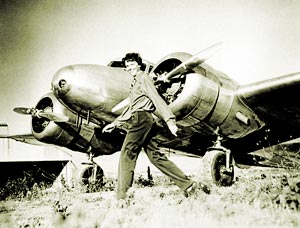
\includegraphics[width = .9\textwidth]{figs/amelia}
\end{frame}

\begin{frame}[fragile]{Run Amelia}
\small
\begin{semiverbatim}
filled <- amelia(data.frame(d) %>%
                   mutate(educ = educ,
                          paeduc = paeduc,
                          race = race,
                          sex = sex),
                 ords = c("paeduc","educ"),
                 noms = c("race","sex"),
                 idvars = "id")
\end{semiverbatim}
\end{frame}

\begin{frame}[fragile]{Run Amelia}
\small
\begin{semiverbatim}
> summary(filled)

Amelia output with 5 imputed datasets.
Return code:  1 
Message:  Normal EM convergence. 

Chain Lengths:
--------------
Imputation 1:  3
Imputation 2:  3
Imputation 3:  3
Imputation 4:  3
Imputation 5:  3
\end{semiverbatim}
\end{frame}

\begin{frame}[fragile]{Run Amelia}
\small
\begin{semiverbatim}
Rows after Listwise Deletion:  1927 
Rows after Imputation:  2630 
Patterns of missingness in the data:  4 

Fraction Missing for original variables: 
-----------------------------------------

       Fraction Missing
id          0.000000000
age         0.000000000
race        0.000000000
sex         0.000000000
paeduc      0.266159696
educ        0.003422053
\end{semiverbatim}
\end{frame}

\begin{frame}{Patterns of missingness}
Amelia told us there were 20 patterns of missignness. What were they? \pause \vskip .2cm
\texttt{missmap(filled)} \pause \vskip .2cm
\begin{center}
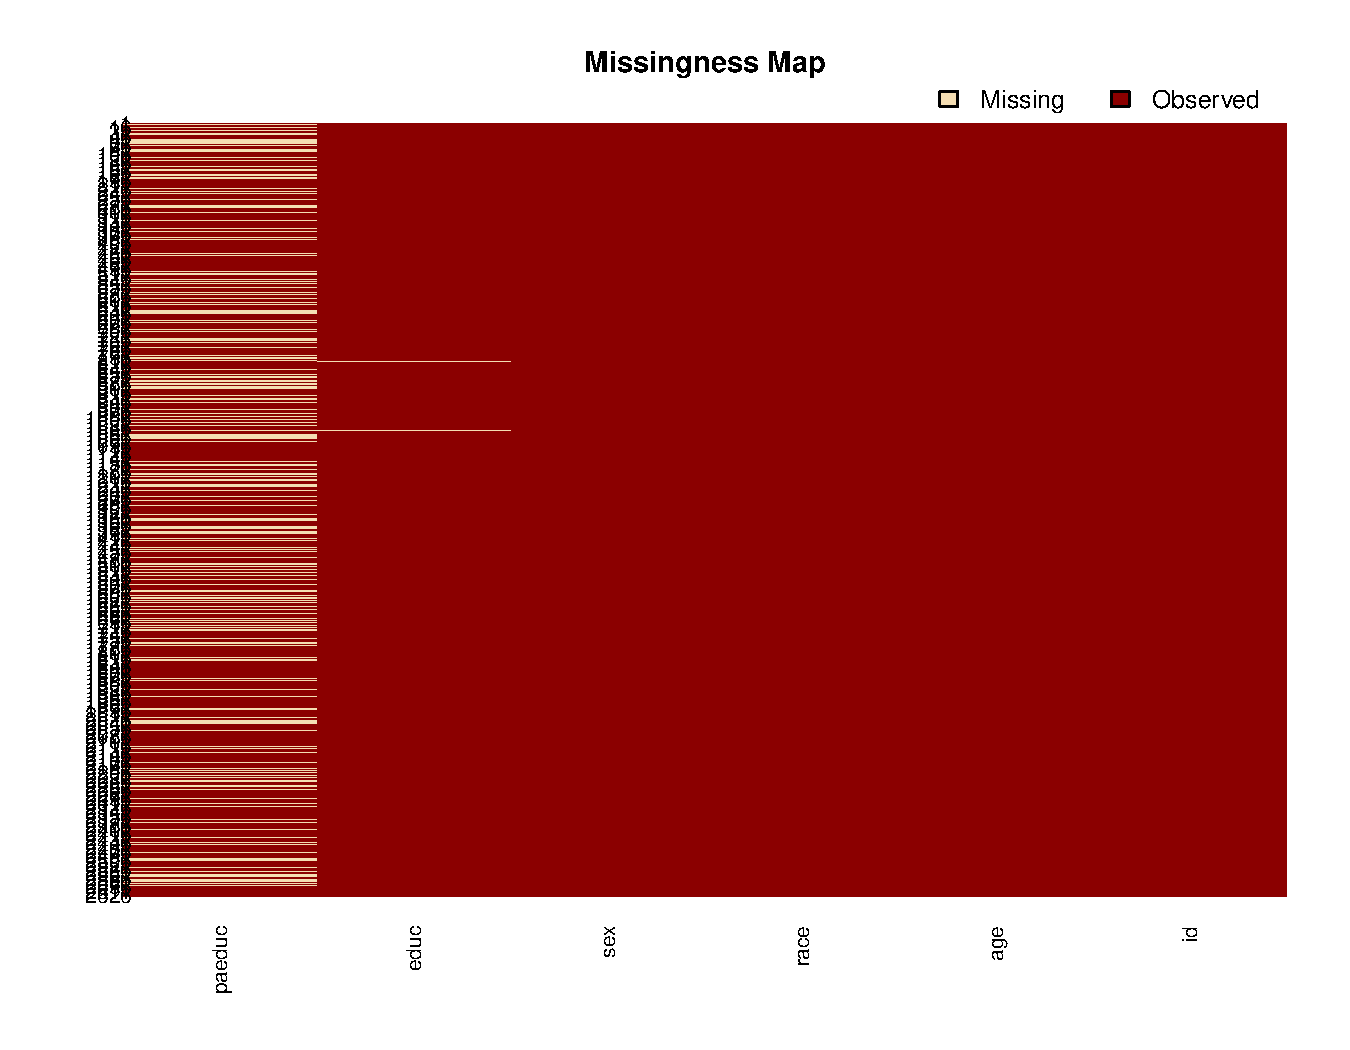
\includegraphics[width = .75\textwidth]{figs/Missmap.pdf}
\end{center}
\end{frame}


%%%%%%NEEEDS UPDATE
%\begin{frame}{Overimputing}
%Overimputing is a check that the imputation model we've set up is doing roughly what we think it's doing. \pause \vskip .5cm
%It does \textcolor{blue}{not} verify the key identification assumption: missing at random. \pause \vskip .5cm
%Idea: \pause
%\begin{itemize}
%\item Knock out some values \pause
%\item Fill in as though they were missing \pause
%\item Compare our imputations to the truth \pause
%\item We want the truth to generally fall in the range of imputed values.
%\end{itemize}
%\end{frame}

%\begin{frame}{Overimputing}
%\texttt{overimpute(filled, var = "paeduc")}
%\begin{center}
%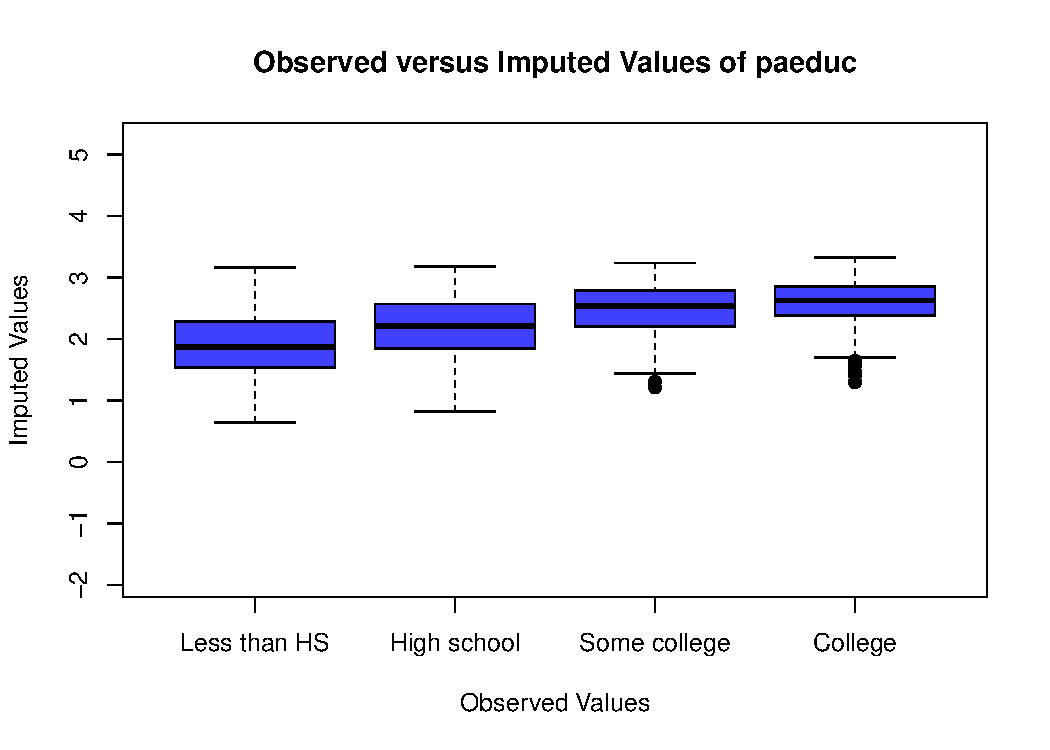
\includegraphics[width = .8\textwidth]{figs/Overimputing.pdf}
%\end{center}
%\end{frame}
%%%%%%%%%END NEEDS UPDATE

\begin{frame}{Checking convergence}
EM can sometimes end up in weird places. \pause \vskip .5cm
We want to know our results converge the same place regardless of the starting values. \pause \vskip .5cm
Amelia's \texttt{disperse()} command shows us that the first principle component (a unidimensional summary of the data) converges to the same value regardless of a few randomly chosen starting points.
\end{frame}

\begin{frame}{Checking convergence}
\texttt{disperse(filled, dims = 1, m = 5)}
\begin{center}
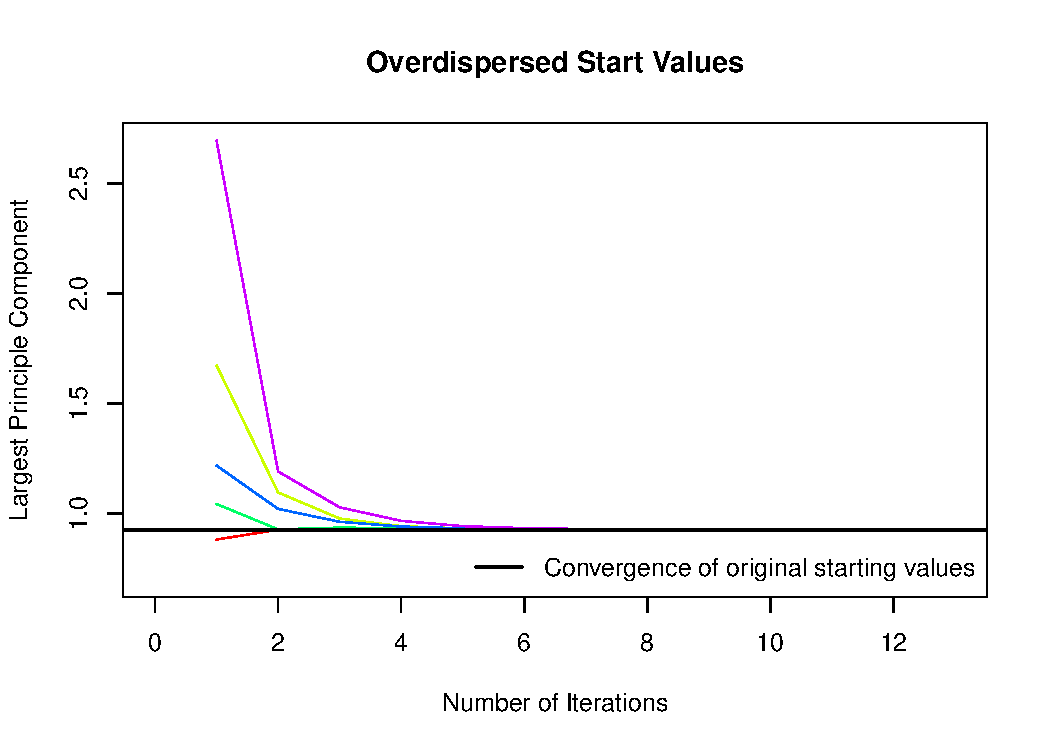
\includegraphics[width = .8\textwidth]{figs/Convergence.pdf}
\end{center}
\end{frame}

\begin{frame}[fragile]{Amelia objects}
Your Amelia object holds lots of things, including 5 versions of the data. \pause
\begin{small}
\begin{semiverbatim}
> head(filled$imputations$imp1)
  id age  race    sex       paeduc         educ
1  1  47 White   Male      College      College
2  2  61 White   Male Less than HS  High school
3  3  72 White   Male  High school      College
4  4  43 White Female Less than HS  High school
5  5  55 White Female      College      College
6  6  53 White Female Less than HS Some college
\end{semiverbatim}
\end{small}
\end{frame}

\begin{frame}[fragile]{\texttt{transform}: Operating on an Amelia object}
What if we now want the respondent's education to be coded as college or not? \pause \textcolor{blue}{\texttt{transform}} operates on all imputations at once. \vskip .5cm \pause
\begin{semiverbatim}
filled_transformed <- transform(
  filled,
  college = (educ == "College")
) \pause
> head(filled_transformed$imputations$imp1)
  id age  race    sex       paeduc         educ college
1  1  47 White   Male      College      College    TRUE
2  2  61 White   Male Less than HS  High school   FALSE
3  3  72 White   Male  High school      College    TRUE
4  4  43 White Female Less than HS  High school   FALSE
5  5  55 White Female      College      College    TRUE
6  6  53 White Female Less than HS Some college   FALSE
\end{semiverbatim}

\end{frame}

\frame{
\frametitle{The Multiple Imputation Scheme (from lecture)}
\hspace{2em}
\begin{tikzpicture}
[overlay,inner sep = 3mm,
missdata/.style={rectangle, draw=red!50, fill=red!20, thick},
 impdata/.style={rectangle, draw=blue!50, fill=blue!20, thick},
results/.style= {circle, draw=blue!50, fill=blue!20, thick}]

\node  (odata) at (3,2) [missdata] {};
\node [red!80,right] at (5.25,2) {incomplete data}; 

\node (imp1) at (1,0) [impdata] {}
  edge [<-, bend left=40] (odata);
\node (imp2) at (2,0) [impdata] {}
  edge [<-, bend left=20] (odata);
\node (imp3) at (3,0) [impdata] {}
  edge [<-] (odata);
\node (imp4) at (4,0) [impdata] {}
  edge [<-, bend right=20] (odata);
\node (imp5) at (5,0) [impdata] {}
  edge [<-, bend right=40] (odata);

\node [blue!80,right] at (5.25,0) {imputed datasets};
\node [black!80, right] at (5.25, 1) {imputation};

\node (res1) at (1,-2) {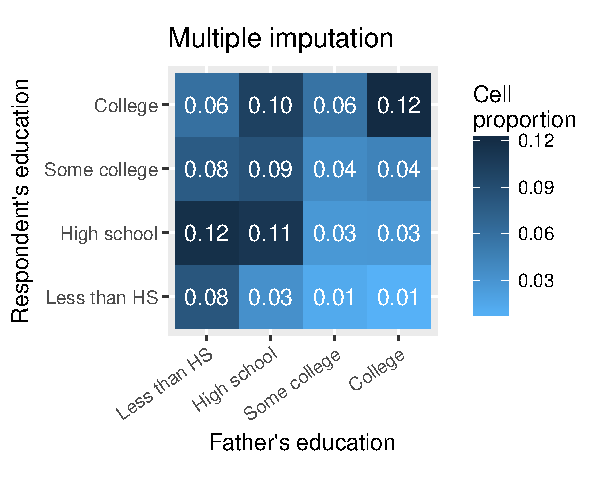
\includegraphics[width = 1cm]{figs/mobility_table_mi1}}
  edge [<-] (imp1);
\node (res2) at (2,-2) {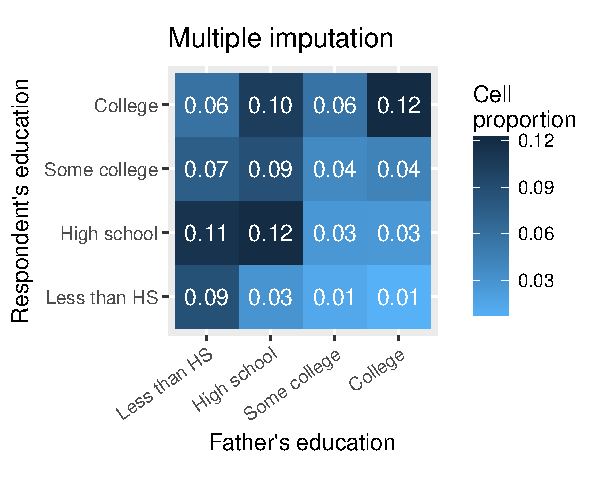
\includegraphics[width = 1cm]{figs/mobility_table_mi2}}
  edge [<-] (imp2);
\node (res3) at (3,-2) {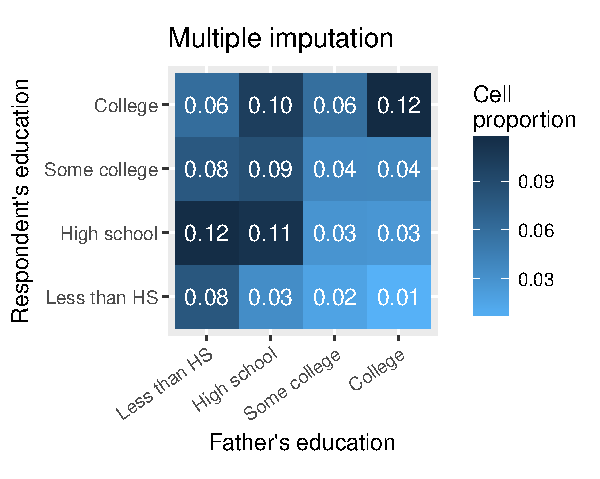
\includegraphics[width = 1cm]{figs/mobility_table_mi3}}
  edge [<-] (imp3);
\node (res4) at (4,-2) {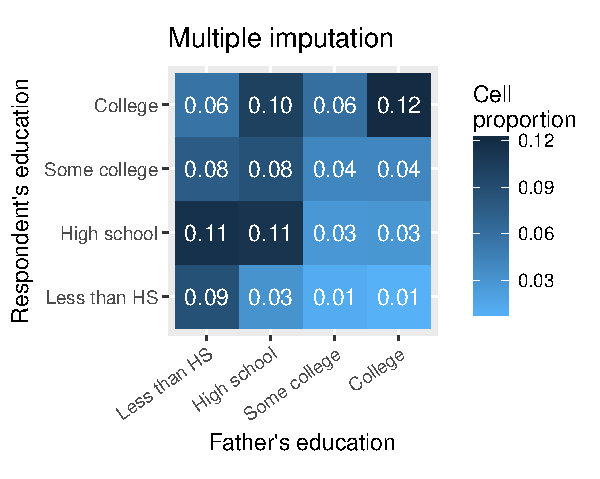
\includegraphics[width = 1cm]{figs/mobility_table_mi4}}
  edge [<-] (imp4);
\node (res5) at (5,-2) {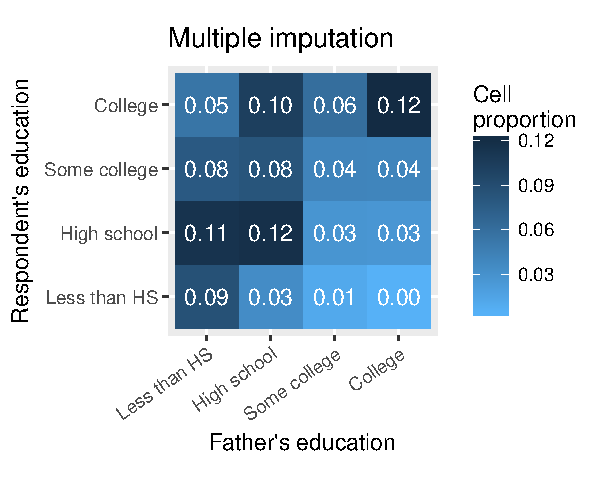
\includegraphics[width = 1cm]{figs/mobility_table_mi5}}
  edge [<-] (imp5);

\node [black!80, right] at (5.25, -1) {analysis};
\node [blue!80, right] at (5.25, -2) {separate results};

\node at (3,-4) {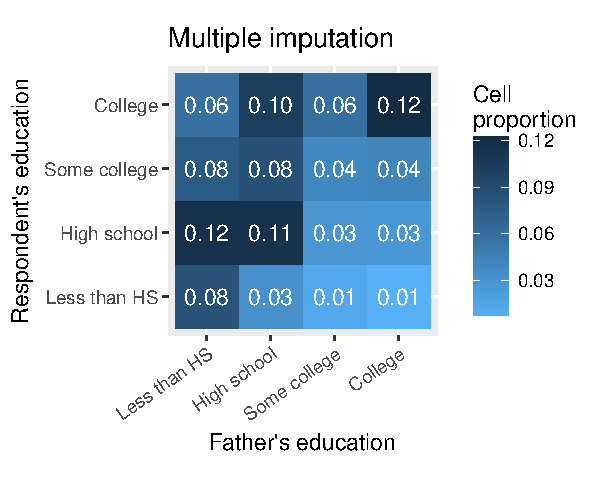
\includegraphics[width = 1cm]{figs/mobility_table_mi}}
  edge [<-, bend right=40] (res5)
  edge [<-, bend left=40] (res1)
  edge [<-, bend right=20] (res4)
  edge [<-, bend left=20] (res2)
  edge [<-] (res3);

\node [black!80, right] at (5.25, -3) {combination};
\node [green!80!black!80, right] at (5.25, -4) { final results};
\end{tikzpicture}

}

\section{Rubin's rules}
\tcframe

\begin{frame}{Combining results: Rubin's rules}

Multiple imputation captures \blue{uncertainty} by combining our uncertainty
\begin{itemize}
\item[--] \bgreen{within} each imputation and 
\item[--] \bgreen{across} imputations.
\end{itemize} \pause
We do this using \blue{Rubin's rules} (idea is important, formula is not).
\begin{center}
\begin{tikzpicture}[x = .5\textwidth, y = .5\textheight]
\node at (0,0) {$\hat\V(\hat\theta) = \underbrace{\frac{1}{m}\sum_{i=1}^m \hat\V(\hat\theta_i)}_{\substack{\text{Mean}\\\text{\bgreen{within-imputation} variance}}} + \underbrace{\left(1 + \frac{1}{m}\right)}_{\substack{\text{Inflation}\\\text{factor}}}\underbrace{\left(\frac{1}{m-1}\sum_{i=1}^m\left[\hat\theta_i - \bar{\hat\theta}\right]\right)}_\text{\bgreen{Between-imputation} variance}$};
\onslide<3->{
\node[blue] (ignored) at (0.1, -.4) {\footnotesize Ignored by single imputation};
\draw[->, line width = 2pt, blue] (ignored) to[bend right = 20] (0.6, -.2);
}
\end{tikzpicture}
\end{center}

\end{frame}

\begin{frame}{Example: Rubin's rules}

Proportion of population with \blue{extreme upward mobility}\\
(father $<$ HS, respondent college)

% latex table generated in R 3.4.3 by xtable 1.8-2 package
% Tue Apr  3 09:14:23 2018
\begin{center}
\begin{tikzpicture}[x = .5\textwidth, y = .5\textheight]
\node at (0,0) {
\begingroup\scriptsize
\begin{tabular}{rll}
  & Proportion & Confidence interval \\ 
   \hline
Imputation 1 & 0.057 & (0.049, 0.066) \\ 
  Imputation 2 & 0.061 & (0.052, 0.070) \\ 
  Imputation 3 & 0.057 & (0.048, 0.065) \\ 
  Imputation 4 & 0.059 & (0.050, 0.068) \\ 
  Imputation 5 & 0.057 & (0.049, 0.066) \\ 
  \end{tabular}
  \endgroup
};
\pause
\node[align=center, font = \footnotesize, blue] (across) at (-.15, -.5) {Uncertainty\\across\\imputations};
\draw[->, thick, blue] (across) -- (-.15, -.25);
\pause
\node[align=center, font = \footnotesize, olive] (within) at (.3, -.5) {Uncertainty\\within each\\imputation};
\draw[->, thick, olive] (within) -- (.3, -.25);
\end{tikzpicture} \\
\onslide<4->{
\large \bgreen{Overall estimate}: 0.058 (0.049, 0.068) \\
The above focuses on intuition.\\The next slides walk through doing this in code.
}
\end{center}
\end{frame}

\begin{frame}[fragile]{In code: Applying Rubin's rules. \blue{Step 1}}
Produce a \blue{list of estimates} from each imputation
\begin{semiverbatim}
estimates <- lapply(filled$imputations, function(imp) \{
  within_imp <- imp %>%
    summarize(proportion = mean(paeduc == 1 & educ == 4))
  return(within_imp$proportion)
\})
\end{semiverbatim}
\end{frame}

\begin{frame}[fragile]{In code: Applying Rubin's rules. \blue{Step 2}}
Produce a \blue{list of the variance} of each imputation-specific estimate
\begin{semiverbatim}
\footnotesize
estimate_variances <- lapply(filled$imputations, function(imp) \{
  within_imp <- imp %>%
    summarize(proportion = mean(paeduc == 1 & educ == 4),
              num = n()) %>%
    mutate(var_proportion = proportion * (1 - proportion) / num)
  return(within_imp$var_proportion)
\})
\end{semiverbatim}
\end{frame}

\begin{frame}[fragile]{In code: Applying Rubin's rules. \blue{Step 3}}
The \texttt{mitools} package has a function \texttt{MIcombine} that \blue{applies Rubin's rules} for you. \vskip .2cm
You give it a list of \blue{results} and a list of \blue{variances} estimated within each imputation. \vskip .2cm
\begin{semiverbatim}
combined <- MIcombine(
  results = estimates,
  variances = estimate_variances
)
\end{semiverbatim}
\end{frame}

\begin{frame}[fragile]{In code: Applying Rubin's rules. \blue{Step 4}}
\blue{Report} the estimate with a 95\% confidence interval.
\begin{semiverbatim}
\footnotesize
combined$coefficients
c(combined$coefficients - qnorm(.975) * sqrt(combined$variance),
  combined$coefficients + qnorm(.975) * sqrt(combined$variance))
\end{semiverbatim}
{\large \bgreen{Overall estimate}: 0.058 (0.049, 0.068)}
\end{frame}

\begin{frame}{All estimators together}
\hspace{2pt}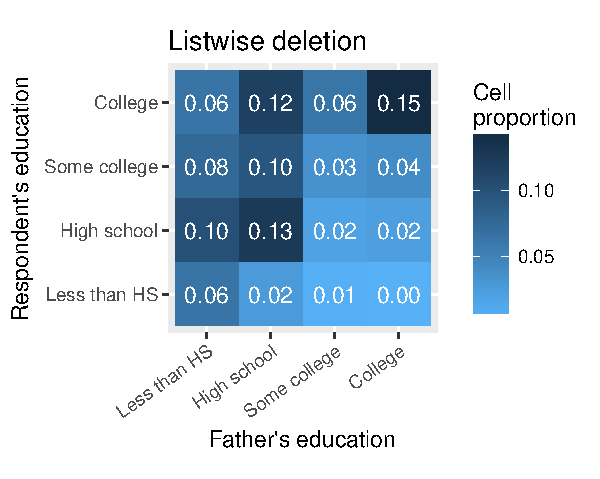
\includegraphics[width = .45\textwidth]{figs/mobility_table_listwise_deletion} \hspace{3pt}
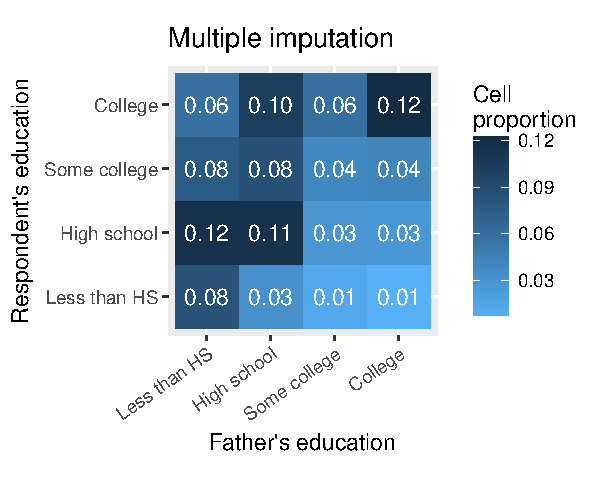
\includegraphics[width = .45\textwidth]{figs/mobility_table_mi} \\
\scalebox{.5625}{\begin{tikzpicture}[x = .5\textwidth, y = .5\textheight]
\node at (0,0) {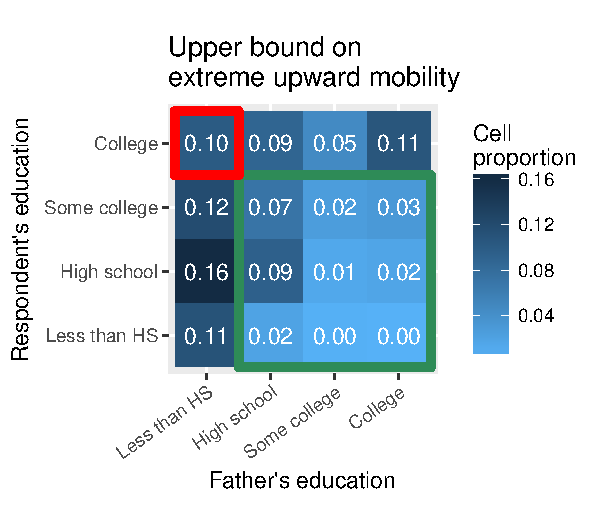
\includegraphics[width = .8\textwidth]{figs/mobility_table_upper_bound}};
\node[red] (upper) at (-.6,.65) {\textbf{Upper bound}};
\draw[->, red, line width = 2pt] (upper) to[bend right] (-.38,.47);
\node[olive] (lower) at (.55,-.5) {\textbf{Lower bound}};
\draw[->, olive, line width = 2pt] (lower) to[bend right] (.4,-.3);
\end{tikzpicture}}
\scalebox{.5625}{\begin{tikzpicture}[x = .5\textwidth, y = .5\textheight]
\node at (0,0) {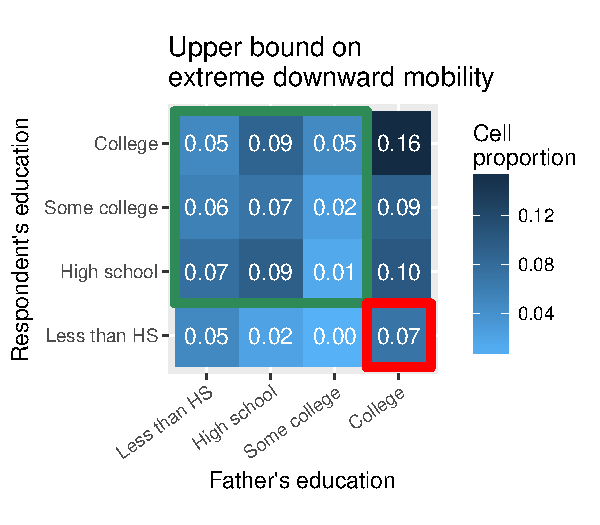
\includegraphics[width = .8\textwidth]{figs/mobility_table_lower_bound}};
\node[olive] (upper) at (-.6,.65) {\textbf{Lower bound}};
\draw[->, olive, line width = 2pt] (upper) to[bend right] (-.38,.47);
\node[red] (lower) at (.55,-.5) {\textbf{Upper bound}};
\draw[->, red, line width = 2pt] (lower) to[bend right] (.4,-.3);
\end{tikzpicture}}
%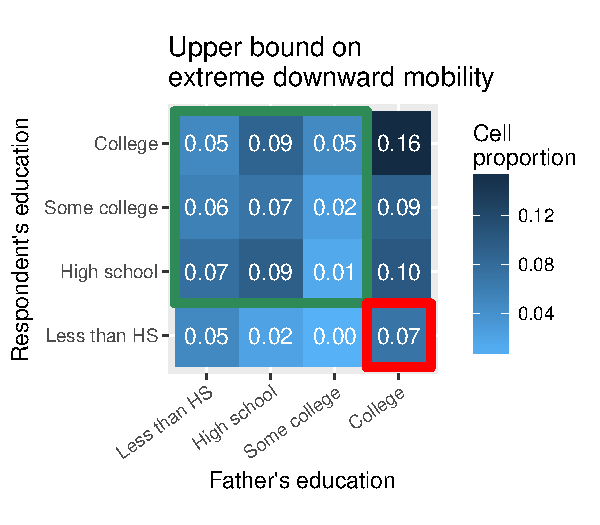
\includegraphics[width = .45\textwidth]{figs/mobility_table_lower_bound}
%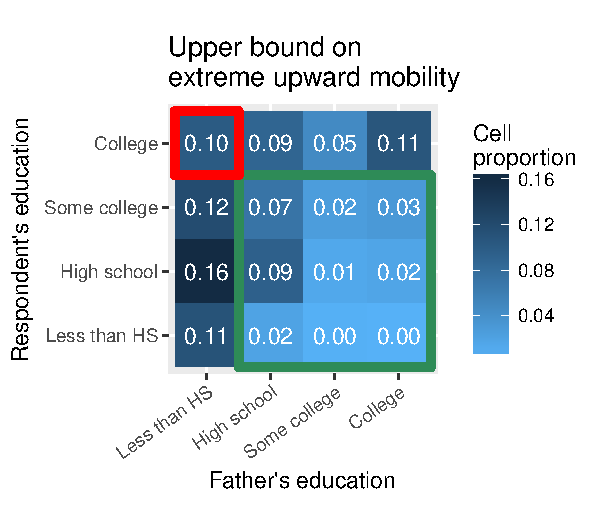
\includegraphics[width = .45\textwidth]{figs/mobility_table_upper_bound}
\end{frame}

\section{Simulation}
\tcframe


\begin{frame}{Combining by simulation}

We can do the same thing by \bblue{simulation}.

\begin{enumerate}
\item On each imputation $j = 1,\dots,m$
\begin{enumerate}
\item Fit a model
\item Store your estimate $\hat\tau_j = h\left(\vec{\hat\theta}_j\right)$
\item Draw $r = 1,000$ simulations
\end{enumerate}
\item Report your \bgreen{point estimate}:
$$\hat\tau = \frac{1}{m}\sum_{j=1}^m \hat\tau_j$$
\item Report \bgreen{uncertainty}
\begin{enumerate}
\item \bblue{Pool} all the simulations.
\item Report a 95\% quantile-based confidence interval
\end{enumerate}
\end{enumerate}

\end{frame}

\begin{frame}{Combining by simulation: \blue{Step 1. Fit a model}}
\begin{center}
\begin{tikzpicture}[x = .5\textwidth, y = .5\textheight]
\node at (0,0) {$\begin{aligned}
Y_i &\sim \text{Bernoulli}(\pi_i) \\
\logit(\pi_i) &= \vec{X}_i\vec\beta
\end{aligned}$};
\node[font = \footnotesize, olive] (college) at (-.15, .32) {College completion};
\draw[->, thick, olive] (college) -- (-.15, .13);
\node[font = \footnotesize, olive] (paeduc) at (0.02, -.3) {Father's education};
\draw[->, thick, olive] (paeduc) -- (0.015, -.14);
\end{tikzpicture}
\end{center}
Store our estimate $\hat\tau_j = \logit^{-1}\left(x\hat{\vec\beta}_j\right)$ \vskip .2cm
Draw 1,000 samples of our quantity of interest
$$\tilde{\vec\beta} \sim \text{Normal}\left(\hat{\vec\beta}, \hat\V\left(\hat{\vec\beta}\right)\right))$$
$$\tilde\tau_{j[r]} = \logit^{-1}\left(x\tilde{\vec\beta}_j\right)$$
\end{frame}

\begin{frame}[fragile]{Combining by simulation: \blue{Step 1. Fit a model}}
\footnotesize \pause
\begin{semiverbatim}
r <- 1000 \pause
setx <- c(1,0,0,0) \pause
fits <- foreach(i = 1:length(filled_transformed$imputations)) %do% \{ \pause
  fit <- glm(college ~ paeduc,
             data = filled_transformed$imputations[[i]],
             family = binomial(link = "logit")) \pause
  estimate <- plogis(setx %*% coef(fit)) \pause
  sim_beta <- rmvnorm(r, mean = coef(fit), sigma = vcov(fit)) \pause
  simulations <- plogis(setx %*% t(sim_beta)) \pause
  return(list(estimate = estimate,
              simulations = simulations))
\}
\end{semiverbatim}
\end{frame}

\begin{frame}[fragile]{Combining by simulation: \blue{Step 2. Report a point estimate}}
This is the same as with Rubin's rules: \\
\bgreen{average} the imputation-specific estimates.
$$\hat\tau = \frac{1}{m}\sum_{j=1}^m \hat\tau_j$$ \pause
$$\begin{aligned}
\hat\P(\text{College}\mid \text{Father} < \text{HS}) &= \frac{1}{m}\sum_{i=1}^m \hat\tau_j \\
&= \frac{1}{5}(0.18 + 0.17 + 0.18 + 0.17 + 0.16) \\
&= 0.17
\end{aligned}$$ \pause
\begin{semiverbatim} \footnotesize
estimate <- mean(sapply(fits, function(fit) fit$estimate))
\end{semiverbatim}
\end{frame}

\begin{frame}[fragile]{Combining by simulation: \blue{Step 3. Report uncertainty}}
\bgreen{Pool} all simulations
$$\tilde\tau = \begin{bmatrix} \tilde\tau_1 \\ \vdots \\ \tilde\tau_m \end{bmatrix}$$ \pause
Report a quantile-based confidence interval
$$\left(\tilde\tau_{(.025)}, \tilde\tau_{(.975)}\right) = (0.15, 0.20)$$ \pause
\begin{semiverbatim} \footnotesize
pooled_simulations <- do.call(
  c,
  lapply(fits, function(fit) fit$simulations)
)
ci <- quantile(pooled_simulations, c(.025, .975))
\end{semiverbatim}
\end{frame}

\section{Review}

\frame{
\frametitle{The Multiple Imputation Scheme (again)}
\hspace{2em}
\pause
\begin{tikzpicture}
[overlay,inner sep = 3mm,
missdata/.style={rectangle, draw=red!50, fill=red!20, thick},
 impdata/.style={rectangle, draw=blue!50, fill=blue!20, thick},
results/.style= {circle, draw=blue!50, fill=blue!20, thick}]

\node  (odata) at (3,2) [missdata] {};
\node [red!80,right] at (5.25,2) {incomplete data}; 

\pause
\node (imp1) at (1,0) [impdata] {}
  edge [<-, bend left=40] (odata);
\node (imp2) at (2,0) [impdata] {}
  edge [<-, bend left=20] (odata);
\node (imp3) at (3,0) [impdata] {}
  edge [<-] (odata);
\node (imp4) at (4,0) [impdata] {}
  edge [<-, bend right=20] (odata);
\node (imp5) at (5,0) [impdata] {}
  edge [<-, bend right=40] (odata);

\node [blue!80,right] at (5.25,0) {imputed datasets};
\node [black!80, right] at (5.25, 1) {imputation};

\pause

\node (res1) at (1,-2) [results] {}
  edge [<-] (imp1);
\node (res2) at (2,-2) [results] {}
  edge [<-] (imp2);
\node (res3) at (3,-2) [results] {}
  edge [<-] (imp3);
\node (res4) at (4,-2) [results] {}
  edge [<-] (imp4);
\node (res5) at (5,-2) [results] {}
  edge [<-] (imp5);

\node [black!80, right] at (5.25, -1) {analysis};
\node [blue!80, right] at (5.25, -2) {separate results};

\pause
\node[circle, draw=green!50!black!50, fill=green!20, thick] at (3,-4) {}
  edge [<-, bend right=40] (res5)
  edge [<-, bend left=40] (res1)
  edge [<-, bend right=20] (res4)
  edge [<-, bend left=20] (res2)
  edge [<-] (res3);

\node [black!80, right] at (5.25, -3) {combination};
\node [green!80!black!80, right] at (5.25, -4) { final results};
\end{tikzpicture}

}


\begin{frame}
  \frametitle<+->{Missingness Assumptions (adapted from lecture)}
  \begin{enumerate}[<+->][1.]
  \item \alert{MCAR}: Missing Completely At Random (\textcolor{blue}{naive})
    \begin{equation*}
      \uncover<+->{P(M|X) = P(M)}
    \end{equation*} 
    \uncover<+->{\small Missingness ($M$) is unrelated to father's education ($X$)}
  \item \alert{MAR}: Missing At Random (\textcolor{blue}{empirical})
    \begin{equation*}
      \uncover<+->{P(M|X,Z) = P(M|Z)}
    \end{equation*}
  \uncover<+->{\scriptsize Missingness is not a function of the missing variable ($X$ = Father's education), conditional on measured variables ($Z$ = Mother's education) \\
  e.g., Children with lesser-educated mothers are more likely to have missing fathers}
  \item \alert{NI}: Non-ignorable (\textcolor{blue}{fatalistic}) \\
  $P(M|X)$ doesn't simplify \\
  \uncover<+->{\scriptsize e.g., within cells of mother's education, missingness is still related to father's education \\
  Adding variables to predict father's education can change NI to MAR}
  \end{enumerate}
\end{frame}

\begin{frame}{Assumptions in actual sociology research}
\large

Next, we will discuss these assumptions in the context of \blue{real publications}. \vskip .5cm
I will walk through an example from AJS. \vskip .5cm
Then in groups you will do the same thing for 4 papers from the current issue of ASR. \vskip .5cm
We will highlight \bgreen{what they do well} as well as \blue{things we might do differently}. Remember these are very good papers!
\end{frame}

\begin{frame}{Assumptions in actual sociology research}
In groups, take 10 minutes to discuss the ways missing data were addressed in actual papers. \vskip .5cm
Then summarize for the class:
\begin{itemize}
\item Broadly what the paper argues (very brief)
\item The missing data problem in the paper
\item How the authors addressed it
\item Whether this was appropriate
\item Any other information you wish the author provided
\item What you would do
\end{itemize}
\end{frame}

\begin{withoutheadline}
\begin{frame}
\includegraphics[page = 1, width = \textwidth, trim = 40 0 40 80, clip = T]{Alexander_et_al_2007/paper}
\end{frame}
\begin{frame}
\centering
\includegraphics[width = .7\textwidth]<1-1| handout:1>{Alexander_et_al_2007/Alexander1}
\includegraphics[width = .7\textwidth]<2-2| handout:2>{Alexander_et_al_2007/Alexander2}
\includegraphics[width = .7\textwidth]<3-3| handout:3>{Alexander_et_al_2007/Alexander3}
\includegraphics[width = .7\textwidth]<4-4| handout:4>{Alexander_et_al_2007/Alexander4}
\includegraphics[width = .7\textwidth]<5-5| handout:5>{Alexander_et_al_2007/Alexander5}
\end{frame}
\end{withoutheadline}

\frame{
\frametitle{The Multiple Imputation Scheme (again)}
\begin{tikzpicture}
[overlay,inner sep = 3mm,
missdata/.style={rectangle, draw=red!50, fill=red!20, thick},
 impdata/.style={rectangle, draw=blue!50, fill=blue!20, thick},
results/.style= {circle, draw=blue!50, fill=blue!20, thick}]

\node  (odata) at (3,2) [missdata] {};
\node [red!80,right] at (5.25,2) {incomplete data}; 

\node (imp1) at (1,0) [impdata] {}
  edge [<-, bend left=40] (odata);
\node (imp2) at (2,0) [impdata] {}
  edge [<-, bend left=20] (odata);
\node (imp3) at (3,0) [impdata] {}
  edge [<-] (odata);
\node (imp4) at (4,0) [impdata] {}
  edge [<-, bend right=20] (odata);
\node (imp5) at (5,0) [impdata] {}
  edge [<-, bend right=40] (odata);

\node [blue!80,right] at (5.25,0) {imputed datasets};
\node [black!80, right] at (5.25, 1) {imputation};

\node (res1) at (1,-2) [results] {}
  edge [<-] (imp1);
\node (res2) at (2,-2) [results] {}
  edge [<-] (imp2);
\node (res3) at (3,-2) [results] {}
  edge [<-] (imp3);
\node (res4) at (4,-2) [results] {}
  edge [<-] (imp4);
\node (res5) at (5,-2) [results] {}
  edge [<-] (imp5);

\node [black!80, right] at (5.25, -1) {analysis};
\node [blue!80, right] at (5.25, -2) {separate results};

\node[circle, draw=green!50!black!50, fill=green!20, thick] at (3,-4) {}
  edge [<-, bend right=40] (res5)
  edge [<-, bend left=40] (res1)
  edge [<-, bend right=20] (res4)
  edge [<-, bend left=20] (res2)
  edge [<-] (res3);

\node [black!80, right] at (5.25, -3) {combination};
\node [green!80!black!80, right] at (5.25, -4) { final results};
\end{tikzpicture}

}


\begin{frame}{Assumptions in actual sociology research}
In groups, take 10 minutes to discuss the ways missing data were addressed in actual papers. \vskip .5cm
Then summarize for the class:
\begin{itemize}
\item Broadly what the paper argues (very brief)
\item The missing data problem in the paper
\item How the authors addressed it
\item Whether this was appropriate
\item Any other information you wish the author provided
\item What you would do
\end{itemize}
\end{frame}

\begin{withoutheadline}
%\begin{frame}
%\includegraphics[page = 1, width = \textwidth, trim = 40 0 40 60, clip = T]{ASR_current/Wilmers_2018}
%\end{frame}
%\begin{frame}
%\includegraphics[page = 1, width = \textwidth, trim = 40 0 40 80, clip = T]{ASR_current/Freeland_Hoey_2018}
%\end{frame}
\begin{frame}
\includegraphics[page = 1, width = \textwidth, trim = 40 0 40 70, clip = T]{ASR_current/Liu_2018}
\end{frame}
\begin{frame}
\centering
\includegraphics<1-1| handout:1>[width = .7\textwidth]{ASR_current/Liu1} \vskip .05cm
\includegraphics<1-1| handout:1>[width = .7\textwidth]{ASR_current/Liu2}
\includegraphics<2-2| handout:2>[width = .7\textwidth]{ASR_current/Liu3}
\end{frame}
\begin{frame}
\includegraphics[page = 1, width = \textwidth, trim = 40 0 40 80, clip = T]{ASR_current/Mize_Manago_2018}
\end{frame}
\begin{frame}
\centering
\includegraphics<1-1| handout:1>[width = .7\textwidth]{ASR_current/Mize0}
\includegraphics<2-2| handout:2>[width = .7\textwidth]{ASR_current/Mize1} \vskip .05cm
\includegraphics<2-2| handout:2>[width = .7\textwidth]{ASR_current/Mize2}
\includegraphics<3-3| handout:3>[width = \textwidth]{ASR_current/Mize3}
\end{frame}
\begin{frame}
\includegraphics[page = 1, width = \textwidth, trim = 40 0 40 80, clip = T]{ASR_current/Quadlin_2018}
\end{frame}
\begin{frame}
\centering
\includegraphics<1-1| handout:1>[width = .7\textwidth]{ASR_current/Quadlin1} \vskip .05cm
\includegraphics<1-1| handout:1>[width = .7\textwidth]{ASR_current/Quadlin2}
\includegraphics<2-2| handout:2>[width = .7\textwidth]{ASR_current/Quadlin3}
\end{frame}
\begin{frame}
\includegraphics[page = 1, width = \textwidth, trim = 40 0 40 80, clip = T]{ASR_current/Kadivar_2018}
\end{frame}
\begin{frame}
\centering
\includegraphics<1-1| handout:1>[width = .7\textwidth]{ASR_current/Kadivar1} \vskip .05cm
\includegraphics<1-1| handout:1>[width = .7\textwidth]{ASR_current/Kadivar2}
\includegraphics<2-2| handout:2>[width = .7\textwidth]{ASR_current/Kadivar3}
\end{frame}
\end{withoutheadline}

\begin{frame}{Revisiting our goals}
By the end of precept, you should be able to:
\begin{enumerate}
\item Feel comfortable with three common \bgreen{assumptions} about missing data
\begin{itemize}
\item Missing completely at random
\item Missing at random
\item Non-ignorable
\end{itemize}
\item Be able to reason about the plausibility of these assumptions using \bgreen{substantive knowledge} in real research settings.
\item Connect assumptions to concrete \bgreen{strategies} to deal with missing data
\begin{itemize}
\item Listwise deletion
\item Multiple imputation
\item Bounds
\end{itemize}
\end{enumerate}
\end{frame}

\begin{frame}[fragile]
\begin{center}
As you leave: Handout on poster and paper writing. \\
Next week: Design-based sampling. \\
\bigskip
\Large \bblue{Cards!} \bgreen{Questions?} \\ \bigskip

\includegraphics[width = .5\textwidth]{figs/single_plane}
\end{center}
\end{frame}


\section[EM]{Bonus slides to help with optional homework problem: EM}
\tcframe

\begin{frame}{Mixture of exponentials}
\centering
$$\begin{aligned}
X_{0i}&\sim \text{Exponential}(\lambda_0) \\ \pause
X_{1i}&\sim \text{Exponential}(\lambda_1) \\ \pause
Z_i &\sim \text{Bernoulli}(p) \\ \pause
Y_i &\equiv (1 - Z_i)X_{0i} + Z_iX_{1i}
\end{aligned}$$
We observe $Y_i$ but $Z_i$ is \bblue{latent}: unobserved. \\
When there is a latent variable, you should think \bgreen{EM}!
\end{frame}

\begin{frame}[fragile]{Simulate the data}
We'll simulate some fake data and try to recover the parameters.
\begin{semiverbatim}
set.seed(08544) \pause
x0 <- rexp(100, rate = 0.5) \pause
x1 <- rexp(100, rate = 2) \pause
z <- rbinom(100, size = 1, prob = .6) \pause
y <- (1 - z)*x0 + z*x1
\end{semiverbatim}
\end{frame}

\begin{frame}{Distribution within each (unknown) class $Z$}
\centering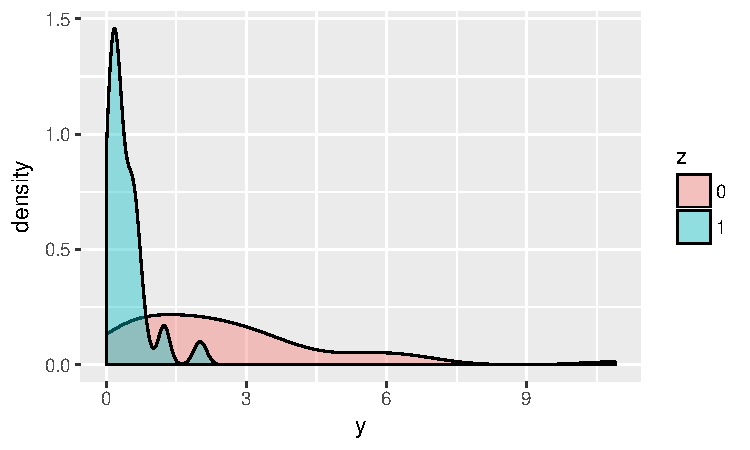
\includegraphics[width = .8\textwidth]{figs/expoMixture1.pdf}
\end{frame}

\begin{frame}{We observe this \blue{marginal} distribution of $Y$}
\centering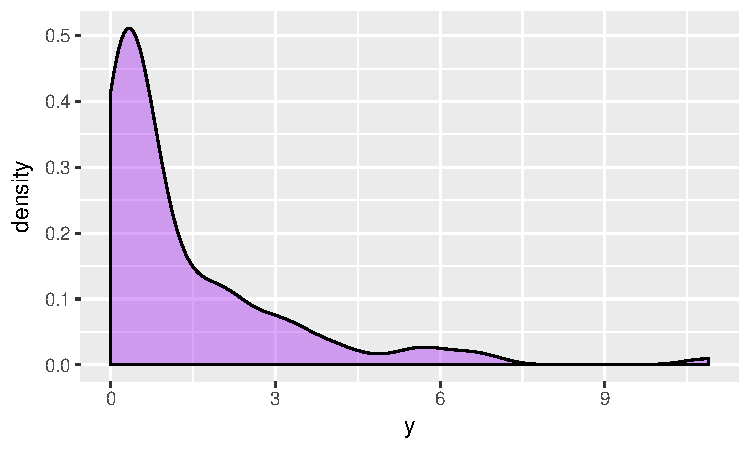
\includegraphics[width = .8\textwidth]{figs/expoMixture2.pdf}
\end{frame}

\begin{frame}{E-step}

Find the expected value of the latent variable $Z_i$, given the parameters $\{p^t,\lambda_0^t,\lambda_1^t\}$ and the data $Y_i$. \vskip .5cm \pause
We sometimes call these the \textcolor{blue}{responsibilities}. \pause

\begin{footnotesize}
$$\begin{aligned}
E(Z_i\mid p^t,\lambda_0^t,\lambda_1^t,Y_i) &=  \pause P(Z_i = 1\mid p^t,\lambda_0^t,\lambda_1^t,Y_i) \\ \pause
&= \frac{P(Y_i\mid Z_i=1)P(Z_i=1)}{P(Y_i)} \\ \pause
&= \frac{P(Y_i\mid Z_i=1)P(Z_i=1)}{P(Y_i\mid Z_i=1)P(Z_i=1) + P(Y_i\mid Z_i=0)P(Z_i=0)} \\ \pause
&= \frac{\lambda_1e^{-y_i\lambda_1}p}{\lambda_1e^{-y_i\lambda_1}p + \lambda_0e^{-y_i\lambda_0}(1-p)} \\
\end{aligned}$$
Note: Conditioning on the parameters is not written explicitly after the first step to simplify the presentation. But all quantities throughout are conditional on $p^t,\lambda_0^t$, and $\lambda_1^t\}$. Likewise, $P$ refers to both probability and probability densities for simplicity.
\end{footnotesize}
\end{frame}

\begin{frame}[fragile]{E-step}
\begin{semiverbatim}
e.step <- function(p, lambda0, lambda1, y) \{
  e.z <- lambda1 * exp(-y * lambda1) * p /
    lambda1 * exp(-y * lambda1) * p + 
    lambda0 * exp(-y * lambda0) * (1 - p)
  return(e.z)
\}
\end{semiverbatim}
\end{frame}

\begin{frame}{M-step}

Find updated MLE estimates of $\{p^t,\lambda_0^t,\lambda_1^t\}$ using the data $z^t$ created in the E-step. \vskip .2cm \pause
First, write the \textcolor{blue}{complete data log likelihood}, which includes both observed and latent variables. \vskip .2cm \pause
\begin{small}
$$\begin{aligned}
L(p^t,\lambda_0^t,\lambda_1^t\mid y,z) &= f(y,z\mid p^t,\lambda_0^t,\lambda_1^t) \\ \pause
&= f(y\mid z,p^t,\lambda_0^t,\lambda_1^t)f(z) \\ \pause
&= \prod_{i=1}^n (\lambda_1e^{-y_i\lambda_1})^{z_i}(\lambda_0e^{-y_i\lambda_0})^{1-z_i}p^{z_i}(1-p)^{1-z_i} \\ \pause
\ell(p^t,\lambda_0^t,\lambda_1^t\mid y,z) &= \sum_{i=1}^n \bigg(z_i(\log\lambda_1 - y_i\lambda_1) \\ \pause
&\qquad + (1-z_i)(\log\lambda_0 - y_i\lambda_0) \\ \pause
&\qquad + z_i\log p_i + (1-z_i)\log(1-p_i)\bigg) \\ \pause
\end{aligned}$$
\end{small}
\end{frame}

\begin{frame}[fragile]{M-step}
\begin{semiverbatim}
comp.data.log.lik <- function(par,z,y) \{ \pause
  p <- plogis(par[1])
  lambda0 <- exp(par[2])
  lambda1 <- exp(par[3]) \pause
  log.lik <- sum(z*(log(lambda1) - y*lambda1) +
                   (1 - z)*(log(lambda0) - y*lambda0) +
                   z*log(p) + (1 - z)*log(1 - p)) 
  return(log.lik)
\}
\end{semiverbatim}
\end{frame}

\begin{frame}[fragile]{M-step}
Write a function to maximize that log likelihood
\begin{semiverbatim}
m.step <- function(z,y) \{ \pause
  opt.out <- optim(
    par = c(0,0,0),
    z = z,
    y = y,
    fn = comp.data.log.lik,
    method = "BFGS",
    control = list(fnscale = -1)
  ) \pause
  p <- plogis(opt.out$par[1])
  lambda0 <- exp(opt.out$par[2])
  lambda1 <- exp(opt.out$par[3])
  return(list(p = p, lambda0 = lambda0,
              lambda1 = lambda1))
\}
\end{semiverbatim}
\end{frame}

\begin{frame}[fragile]{Put E and M together!}
Initialize the matrix to store parameters
\begin{semiverbatim}
par.estimates <- matrix(nrow = 11, ncol = 3)
colnames(par.estimates) <- c("p.t","lambda0.t","lambda1.t")
\end{semiverbatim} \pause

Choose starting values
\begin{semiverbatim}
p.t <- 0.5
lambda0.t <- 1
lambda1.t <- 1
set.seed(12345)
z.t <- rbinom(n = length(y),
              size = 1,
              prob = .5)
\end{semiverbatim} \pause

Store our starting parameters in the matrix
\begin{semiverbatim}
par.estimates[1,] <- c(p.t, lambda0.t, lambda1.t)
\end{semiverbatim}
\end{frame}

\begin{frame}[fragile]{Put E and M together!}
Iterate
\begin{semiverbatim}
for (i in 2:11) \{ \pause
  z.t <- e.step(p = p.t, 
                lambda0 = lambda0.t, 
                lambda1 = lambda1.t,
                y = y) \pause
  
  m.out <- m.step(z = z.t, y = y) \pause
  
  p.t <- m.out$p
  lambda0.t <- m.out$lambda0
  lambda1.t <- m.out$lambda1 \pause
  
  par.estimates[i,] <- c(p.t, lambda0.t, lambda1.t)
\}
\end{semiverbatim}
\end{frame}

\begin{frame}{EM convergence}
\centering
\begin{tabular}{rrrr}
  \hline
Iteration & $p^t$ & $\lambda_0^t$ & $\lambda_1^t$ \\ 
  \hline
0 & 0.5000 & 1.0000 & 1.0000 \\ \pause
  1 & 0.3482 & 0.5409 & 2.7712 \\  \pause
  2 & 0.2474 & 0.6271 & 1.8944 \\  \pause 
  3 & 0.3010 & 0.5934 & 1.9726 \\ \pause
  4 & 0.2779 & 0.6076 & 1.9548 \\ \pause
  5 & 0.2874 & 0.6019 & 1.9603 \\ \pause
  6 & 0.2835 & 0.6042 & 1.9580 \\ \pause
  7 & 0.2851 & 0.6033 & 1.9589 \\ \pause
  8 & 0.2844 & 0.6037 & 1.9585 \\ \pause
  9 & 0.2847 & 0.6035 & 1.9587 \\ \pause
  10 & 0.2846 & 0.6036 & 1.9586 \\ 
   \hline
\end{tabular}
\end{frame}

\end{document}
